% import gaya yang sudah disiapkan
\documentclass{gaya}

% import berbagai variabel
\input{pustaka/variables.tex}
\input{pustaka/jenis-dokumen.tex}

% pemenggalan kata
\input{pustaka/tanda-hubung.tex}

% Isi keseluruhan dokumen
\begin{document}

% Sampul luar bahasa indonesia
\cover
\newpage

% Nomor halaman pembuka dimulai dari sini
\pagenumbering{roman}

% % Sampul dalam bahasa indonesia
% \coverdalam
% \newpage

% % Halaman pengesahan
% \approvalpage
% \cleardoublepage

% % Halaman orisinalitas
% \originalitypage
% \cleardoublepage

% % Halaman publikasi
% \publicationpage
% \cleardoublepage

% !TEX root = ../main.tex
\begin{abstractind}
  \justifying
  Mobilitas kendaraan roda dua yang meningkat di lingkungan perguruan tinggi mempertinggi risiko keselamatan, terutama akibat ketidakpatuhan penggunaan helm. Pengawasan manual yang berlaku saat ini kurang terukur dan belum memberi wawasan spasiotemporal yang presisi sebagai dasar evaluasi kebijakan. Penelitian ini merancang dan mengevaluasi arsitektur pengawasan cerdas berbasis aliran video waktu nyata (\textit{real-time video streaming}) secara ujung ke ujung (\textit{end-to-end}). Arsitektur tersebut memadukan YOLOv8 untuk ekstraksi fitur spasial, ByteTrack untuk pelacakan multiobjek, filter \textit{Intersection over Area} (IoA) dan konfirmasi temporal \textit{N-Frame} untuk menekan deteksi palsu, serta distribusi aliran peristiwa melalui Apache Kafka dan Apache Spark Structured Streaming menuju \textit{data mart} PostgreSQL yang divisualisasikan pada dasbor Grafana. Pada evaluasi eksperimental, model deteksi mencapai \textit{Mean Average Precision} (mAP@50) sebesar 91,4\%; pemrosesan tepi beroperasi stabil pada \textit{throughput} 18,9 FPS dan latensi inferensi 53 milidetik; sedangkan pialang pesan mencatat tingkat keberhasilan pengiriman 100\% dengan median latensi 2,65 milidetik. Pengujian operasional pada data lapangan selama 10 jam (07.00--17.00 WIB) menyaring 11.172 deteksi mentah menjadi 113 kejadian pelanggaran aktual. Dasbor memetakan distribusi kepadatan bimodal dengan puncak anomali tercatat pada pukul 14.45--15.15 WIB yang berkorelasi dengan faktor cuaca dan dinamika pergantian kelas. Infrastruktur terintegrasi tersebut menggeser pengawasan reaktif menjadi instrumen Sistem Pendukung Keputusan (\textit{Decision Support System}) yang proaktif dalam perencanaan patroli keselamatan di lingkungan kampus.

\noindent
\textbf{Kata kunci:} ByteTrack, \textit{Data Mart}, Pelanggaran Helm, YOLOv8 % masukkan keyword
\end{abstractind}

\cleardoublepage

% % Abstrak Bahasa Inggris
% % !TEX root = ../main.tex
\begin{abstracteng}
  \justifying
  The growing mobility of two-wheeled vehicles in university environments raises safety risks, particularly through non-compliance with helmet usage. Existing manual surveillance is hardly scalable and does not provide precise spatio-temporal insights to support policy evaluation. This study designs and evaluates an end-to-end smart surveillance architecture built on real-time video streaming. The architecture combines YOLOv8 for spatial feature extraction, ByteTrack for multi-object tracking, \textit{Intersection over Area} (IoA) filters and \textit{N-Frame} temporal confirmation to suppress false detections, and an event stream that flows through Apache Kafka and Apache Spark Structured Streaming into a PostgreSQL \textit{data mart} that is visualized on an interactive Grafana dashboard. In experimental evaluation, the detection model reaches a \textit{Mean Average Precision} (mAP@50) of 91.4\%; the edge processing pipeline operates stably at 18.9 FPS with 53\,ms inference latency; and the message broker records a 100\% delivery success rate with a 2.65\,ms median latency. Operational testing on 10 hours of field data (07.00--17.00 local time) reduces 11{,}172 raw detections to 113 actual violation events. The dashboard maps a bimodal density distribution, with an anomaly peak recorded at 14:45--15:15 local time that correlates with rainfall and class transition dynamics. The integrated infrastructure shifts reactive surveillance toward a proactive \textit{Decision Support System} that improves the planning of safety patrols in a campus environment.

  \bigskip
  \noindent
  \textbf{Keywords:} YOLOv8, ByteTrack, Stream Processing, Data Mart, Traffic Safety.
\end{abstracteng}

% \cleardoublepage

% % Motto
% \input{lainnya/motto.tex}
% \cleardoublepage

% % Persembahan
% \input{lainnya/halaman-persembahan.tex}
% \cleardoublepage

% % Kata pengantar
% \input{lainnya/kata-pengantar.tex}
% \cleardoublepage

% DAFTAR ISI
\addcontentsline{toc}{chapter}{DAFTAR ISI}
\tableofcontents

% DAFTAR GAMBAR
\phantomsection%<---
\addcontentsline{toc}{chapter}{DAFTAR GAMBAR}
\listoffigures

% DAFTAR TABEL
\phantomsection%<---
\addcontentsline{toc}{chapter}{DAFTAR TABEL}
\listoftables

% % DAFTAR SINGKATAN
% \include{lainnya/daftar-singkatan.tex}

% % DAFTAR SIMBOL
% \include{lainnya/daftar-simbol.tex}

\newpage

% Nomor halaman isi dimulai dari sini
\pagenumbering{arabic}

% BAB 1 PENDAHULUAN
\include{bab/1-pendahuluan.tex}

% % BAB 2 TINJAUAN PUSTAKA
\include{bab/2-tinjauan-pustaka.tex}

% % BAB 3 METODOLOGI PENELITIAN
\include{bab/3-metodologi-penelitian.tex}

% % BAB 4 HASIL DAN PEMBAHASAN
% ============================================================
% BAB IV — HASIL DAN PEMBAHASAN
% ITERA Smart Sentinel: Sistem Deteksi & Analitik Pelanggaran Helm Real-time
% ============================================================

\chapter{HASIL DAN PEMBAHASAN}
\label{chap:hasil}

% ============================================================
\section{Pengembangan Model Deteksi YOLOv8}
\label{sec:model-deteksi}
Subbab ini menguraikan pengembangan model deteksi YOLOv8 untuk atribut keselamatan berkendara di area gerbang kampus. Pembahasan menyusur empat tahap: analisis dataset, pra-pemrosesan dan augmentasi, dinamika pelatihan, serta evaluasi kinerja sebelum model diintegrasikan ke \textit{pipeline} pemrosesan video waktu nyata.

%
\subsection{Eksplorasi Dataset Awal}
\label{subsec:eda-dataset}
%

Analisis eksploratif dilakukan pada dataset mentah hasil tangkapan CCTV. Dataset memuat 390 citra unik berukuran median $1280 \times 720$ piksel dengan total 2.369 anotasi objek atau rata-rata 6,1 anotasi per citra. Tabel~\ref{tab:distribusi-objek} merinci distribusi anotasi pada setiap kelas.

\begin{table}[htbp]
  \centering
  \caption{Jumlah anotasi tiap kelas pada dataset awal.}
  \label{tab:distribusi-objek}
  \begin{tabular}{clc}
    \hline
    \textbf{No.} & \textbf{Kategori Objek} & \textbf{Jumlah Anotasi} \\
    \hline
    0 & \texttt{DRIVER\_HELMET}     & 730 \\
    1 & \texttt{DRIVER\_NO\_HELMET} & 718 \\
    2 & \texttt{MOTORCYCLE}         & 921 \\
    \hline
    \textbf{Total} & & \textbf{2.369} \\
    \hline
  \end{tabular}
\end{table}

Tabel~\ref{tab:distribusi-objek} memuat tiga kelas objek beserta jumlah anotasinya masing-masing. Dua kelas pelanggaran yang menjadi target utama penelitian, yaitu \texttt{DRIVER\_HELMET} (730 anotasi) dan \texttt{DRIVER\_NO\_HELMET} (718 anotasi), hanya berselisih 12 anotasi atau rasio 1{,}02:1, sehingga keduanya dapat dianggap setara. Kesetaraan ini menentukan kualitas diskriminasi model: ketika jumlah sampel antara dua kelas yang harus dibedakan hampir sama, model tidak memiliki alasan statistik untuk berat sebelah ke salah satu kategori. Kelas \texttt{MOTORCYCLE} memperoleh 921 anotasi, sekitar 191--203 lebih banyak daripada dua kelas pelanggaran. Selisih tersebut wajar karena \texttt{MOTORCYCLE} berperan sebagai kelas konteks: badan motor terlihat utuh hampir di setiap citra, sedangkan kepala pengendara kerap tertutup sebagian oleh kaca depan atau penumpang sehingga anotasinya tidak sebanyak anotasi motor.

Suatu dataset mulai dikategorikan mengalami \textit{class imbalance} apabila nilai \textit{imbalance ratio} (IR) melebihi 1,5:1\cite{kraiem2021resampling}. Pada penelitian ini, rasio kelas mayoritas (\texttt{MOTORCYCLE}) terhadap kelas minoritas (\texttt{DRIVER\_NO\_HELMET}) bernilai 921:718 atau 1,28:1, masih di bawah ambang tersebut. Distribusi ketiga kelas dengan demikian tergolong seimbang dan risiko bias model ke kelas mayoritas tergolong rendah.

Selain dari sisi jumlah, kualitas dataset juga dilihat dari posisi kemunculan objek pada bidang pandang kamera. Gambar~\ref{fig:heatmap-per-class} menyajikan peta panas (\textit{annotation heatmap}) anotasi dengan gradasi biru muda hingga merah pekat untuk menggambarkan kepadatan \textit{bounding box} di setiap \textit{grid} citra. Nilai minimum, kuartil pertama, dan median pada legenda sama-sama 0 anotasi, kuartil ketiga 11 anotasi, sedangkan \textit{grid} terpadat memuat 172 anotasi. Angka tersebut menandakan bahwa anotasi terpusat di sebagian kecil area, sementara sebagian besar \textit{grid} citra kosong.

\begin{figure}[htbp]
  \centering
  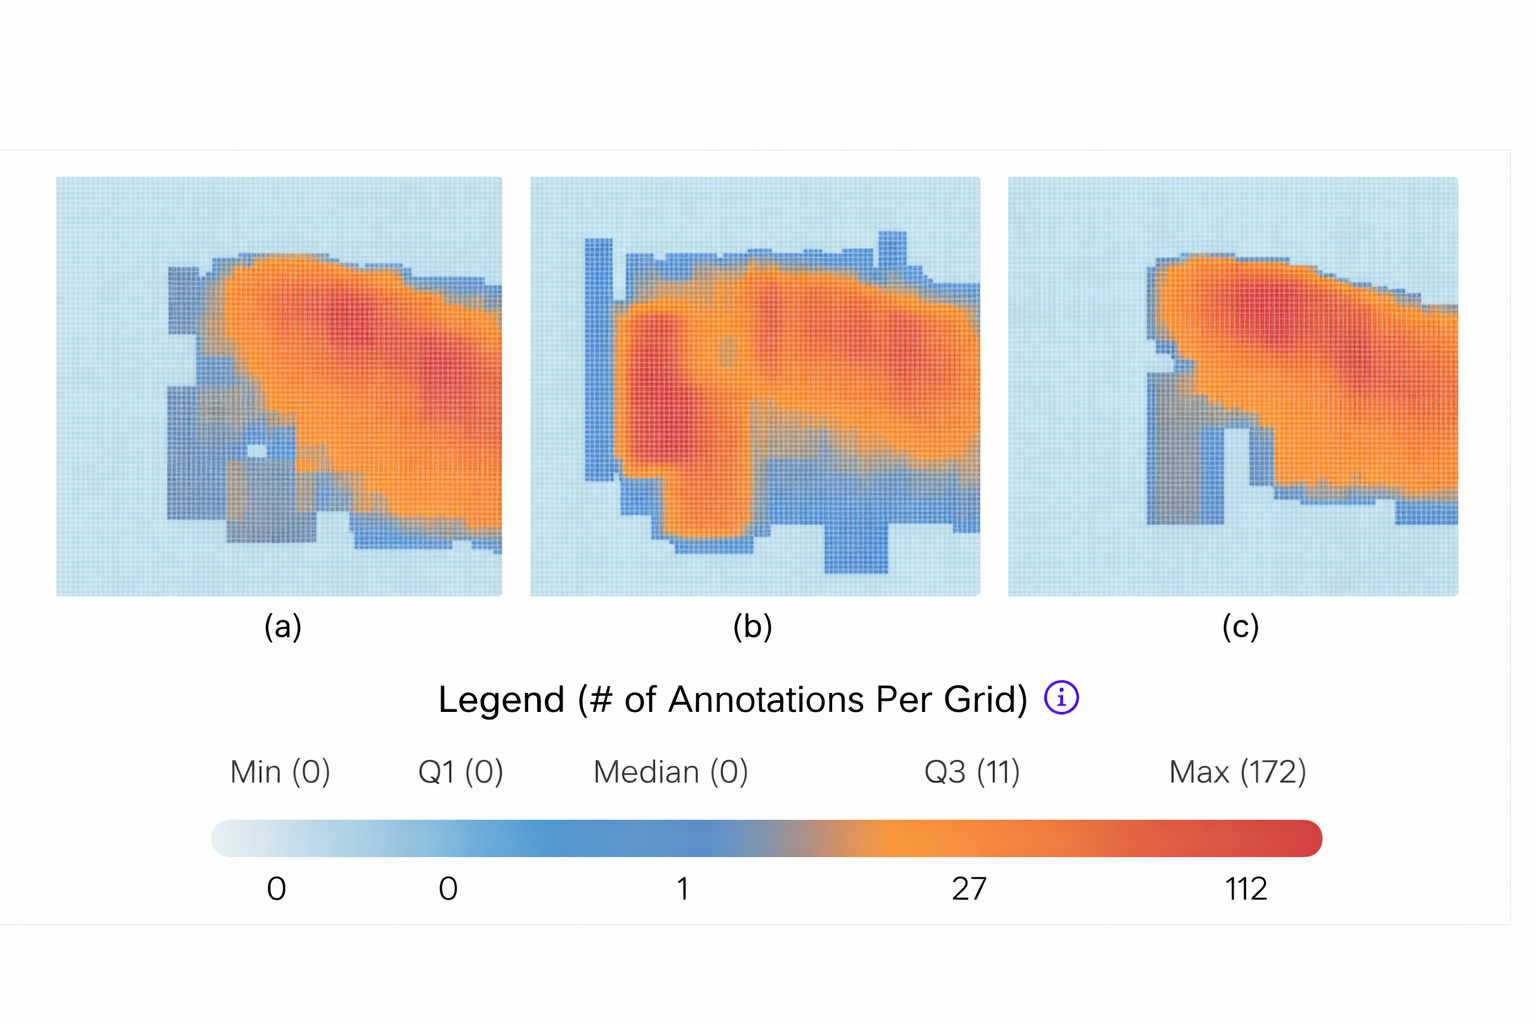
\includegraphics[width=0.95\textwidth]{gambar/heatmap_anotation_class.png}
  \caption{Peta panas (\textit{annotation heatmap}) sebaran anotasi tiap kelas: a) \texttt{DRIVER\_HELMET}, b) \texttt{DRIVER\_NO\_HELMET}, dan c) \texttt{MOTORCYCLE}.}
  \label{fig:heatmap-per-class}
\end{figure}

Pada Gambar~\ref{fig:heatmap-per-class}(a), anotasi kelas \texttt{DRIVER\_HELMET} mengumpul di bagian tengah hingga kanan atas citra dengan titik paling padat tepat di lajur masuk utama. Pola sebaran kelas \texttt{DRIVER\_NO\_HELMET} pada Gambar~\ref{fig:heatmap-per-class}(b) hampir sama, hanya saja zona terpadatnya sedikit bergeser ke arah kiri tengah. Pergeseran ini terjadi karena lajur masuk gerbang Itera lebih lebar di sisi kiri sehingga sebagian pengendara mengambil sisi tersebut. Gambar~\ref{fig:heatmap-per-class}(c) untuk kelas \texttt{MOTORCYCLE} memiliki zona kepadatan yang nyaris sama persis dengan kelas \texttt{DRIVER\_HELMET}, sebab badan motor selalu menyertai pengendara sebagai konteks anotasi. Karena ketiga kelas terpusat pada wilayah yang relatif sama, \textit{Region of Interest} (ROI) ditarik mengikuti kontur jalan dan kira-kira mencakup bagian tengah sampai kanan atas citra.

Di luar ROI, warna peta panas didominasi biru muda hingga abu-abu yang berarti \textit{grid} di area tersebut hampir tidak memuat anotasi. Wilayah ini mencakup langit di bagian atas, trotoar, dan jalur berlawanan di tepi citra. kendaraan dan pengendara tidak melintas di sana sehingga tidak ada \textit{bounding box} yang muncul. Dengan membatasi inferensi pada ROI, area latar yang kosong tidak ikut diproses dan YOLOv8 hanya bekerja di zona yang memang aktif dilewati kendaraan. Cara ini mengurangi beban komputasi sekaligus menaikkan \textit{precision} dan menekan \textit{false positive} saat inferensi waktu nyata.

%
%
\subsection{Pra-pemrosesan dan Augmentasi Data}
\label{subsec:preprocessing-augmentasi}
%

Pra-pemrosesan dan augmentasi mengubah 390 citra mentah menjadi 856 sampel pelatihan terstandarisasi. Setiap citra dikalibrasi dengan \textit{auto-orient}, lalu diubah ukurannya (\textit{resize}) ke resolusi seragam $640 \times 640$ piksel. Tahap augmentasi kemudian menghasilkan tiga variasi sintetis untuk setiap citra asli, dengan rincian hiperparameter pada Tabel~\ref{tab:augmentasi}.


Strategi augmentasi disusun untuk mereplikasi gangguan visual yang lazim terjadi pada kamera pengawas luar ruang. Setiap teknik divisualisasikan dengan citra sebelum dan sesudah augmentasi pada Gambar~\ref{fig:aug-rotasi} sampai Gambar~\ref{fig:aug-noise}, sedangkan parameter \textit{motion blur} dirinci pada Tabel~\ref{tab:augmentasi}.

\begin{figure}[H]
  \centering
  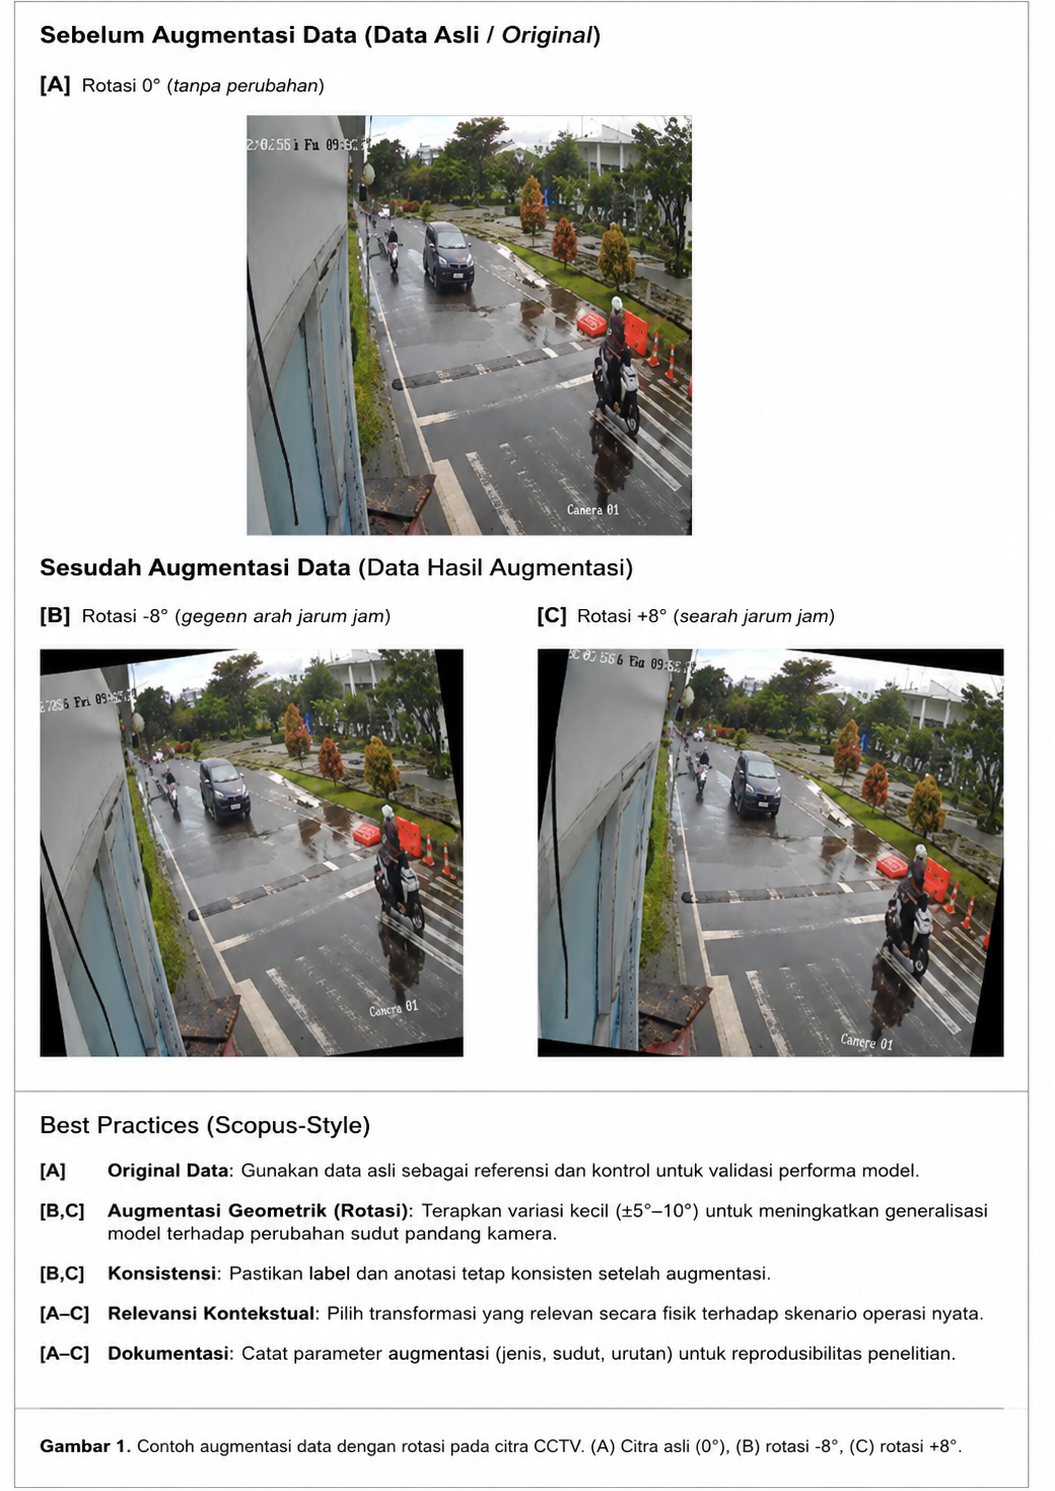
\includegraphics[width=0.85\textwidth]{gambar/aug_rotasi.jpg}
  \caption{Augmentasi rotasi pada rentang $-8^\circ$ sampai $+8^\circ$.}
  \label{fig:aug-rotasi}
\end{figure}

Augmentasi rotasi memutar citra dalam rentang $-8^\circ$ sampai $+8^\circ$ untuk meniru pergeseran sudut tiang kamera akibat getaran atau dorongan angin. Kamera CCTV pada tiang sering kali sedikit miring dari posisi awal sehingga horizon citra ikut berubah. Pelatihan menggunakan citra hasil rotasi membuat model tidak bergantung pada orientasi horizon yang sempurna ketika mengenali pengendara dan motor.

\begin{figure}[H]
  \centering
  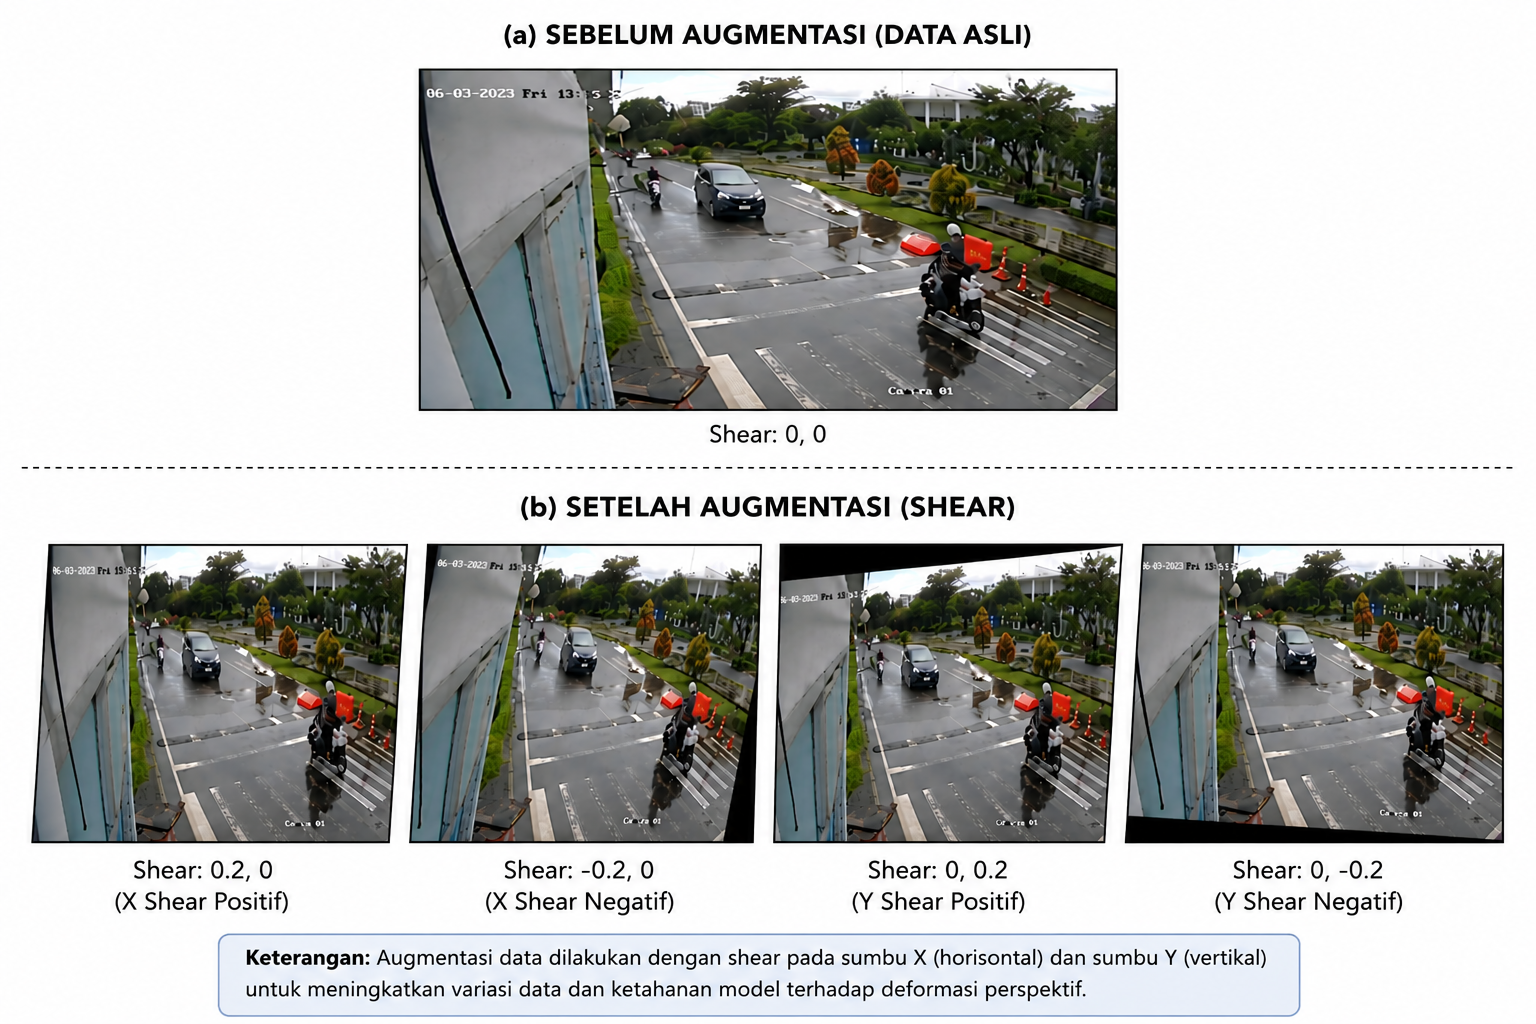
\includegraphics[width=0.95\textwidth]{gambar/aug_shear.jpg}
  \caption{Augmentasi \textit{shear} pada sumbu X dan Y dengan nilai $\pm 0{,}2$.}
  \label{fig:aug-shear}
\end{figure}

Augmentasi \textit{shear} memiringkan citra pada sumbu X dan Y sebesar $\pm 0{,}2$ untuk meniru distorsi perspektif ketika kamera tidak tegak lurus dengan bidang jalan. Empat varian (X positif, X negatif, Y positif, Y negatif) memperluas variasi sudut pandang sehingga model lebih tahan saat sudut pandang kamera di lapangan berbeda dari sudut pelatihan.

\begin{figure}[H]
  \centering
  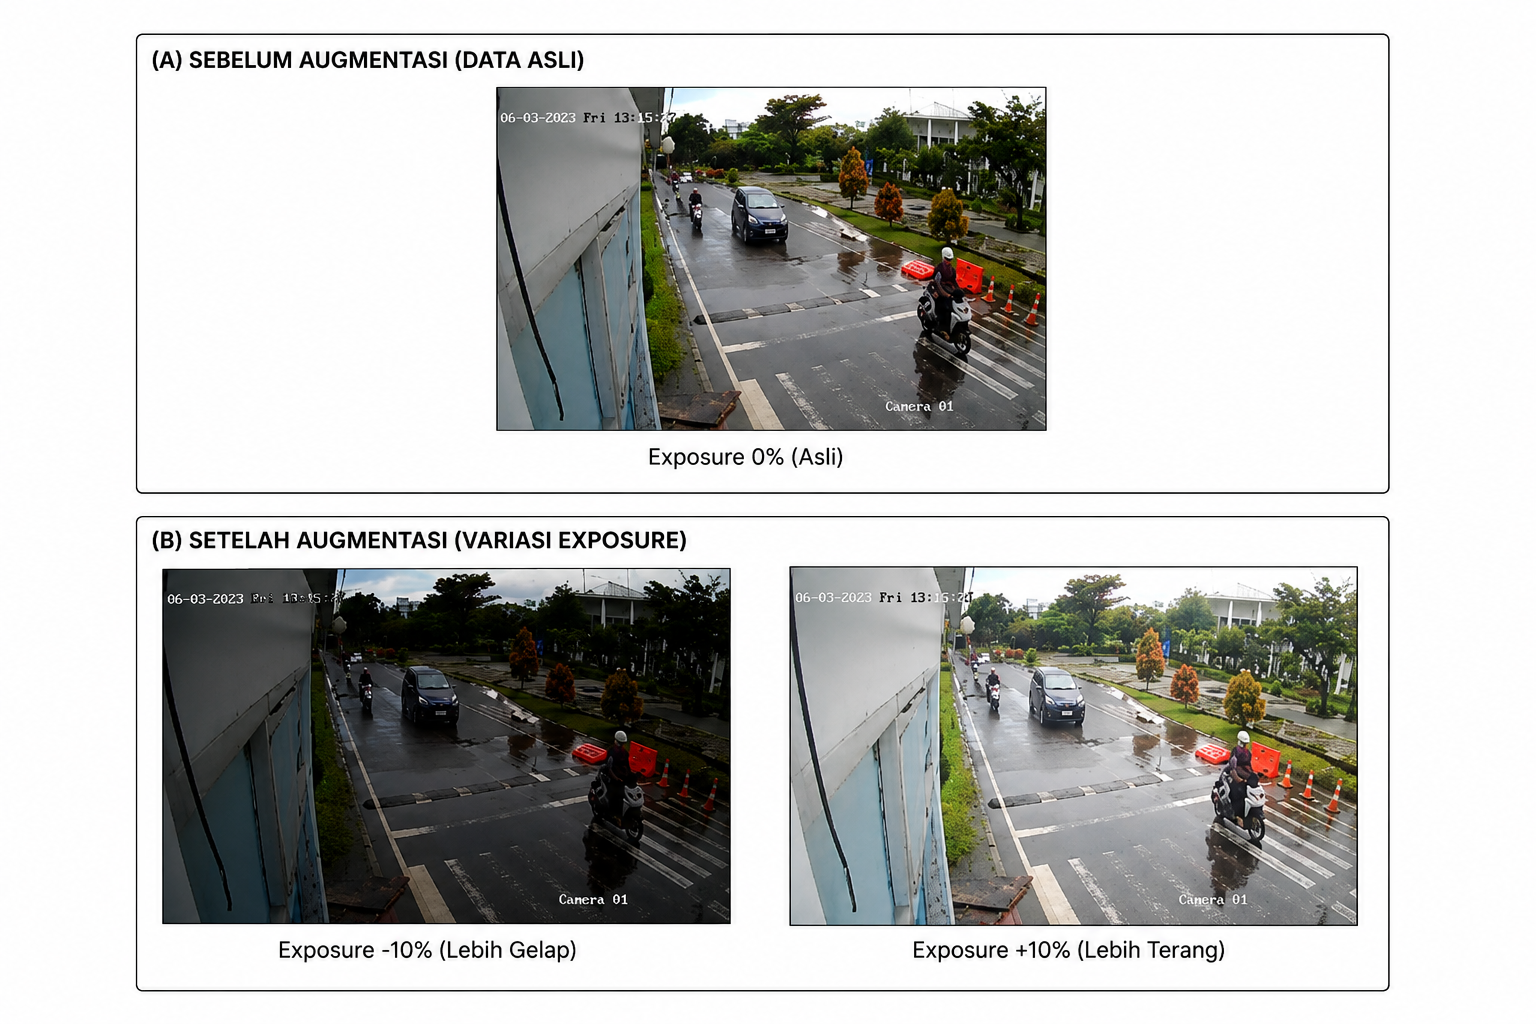
\includegraphics[width=0.95\textwidth]{gambar/aug_exposure.jpg}
  \caption{Augmentasi \textit{exposure} pada rentang $-10\%$ sampai $+10\%$.}
  \label{fig:aug-exposure}
\end{figure}

Variasi \textit{exposure} sebesar $\pm 10\%$ menyimulasikan perubahan iluminasi sepanjang hari, dari pagi yang masih gelap sampai siang yang sangat terang. Citra dengan eksposur $-10\%$ terlihat lebih gelap dengan bayangan yang dominan, sedangkan eksposur $+10\%$ membuat citra lebih cerah dan kontras tampak menurun. Variasi ini menekan ketergantungan model pada nilai kecerahan tertentu sehingga deteksi tetap stabil di berbagai kondisi pencahayaan.

\begin{figure}[H]
  \centering
  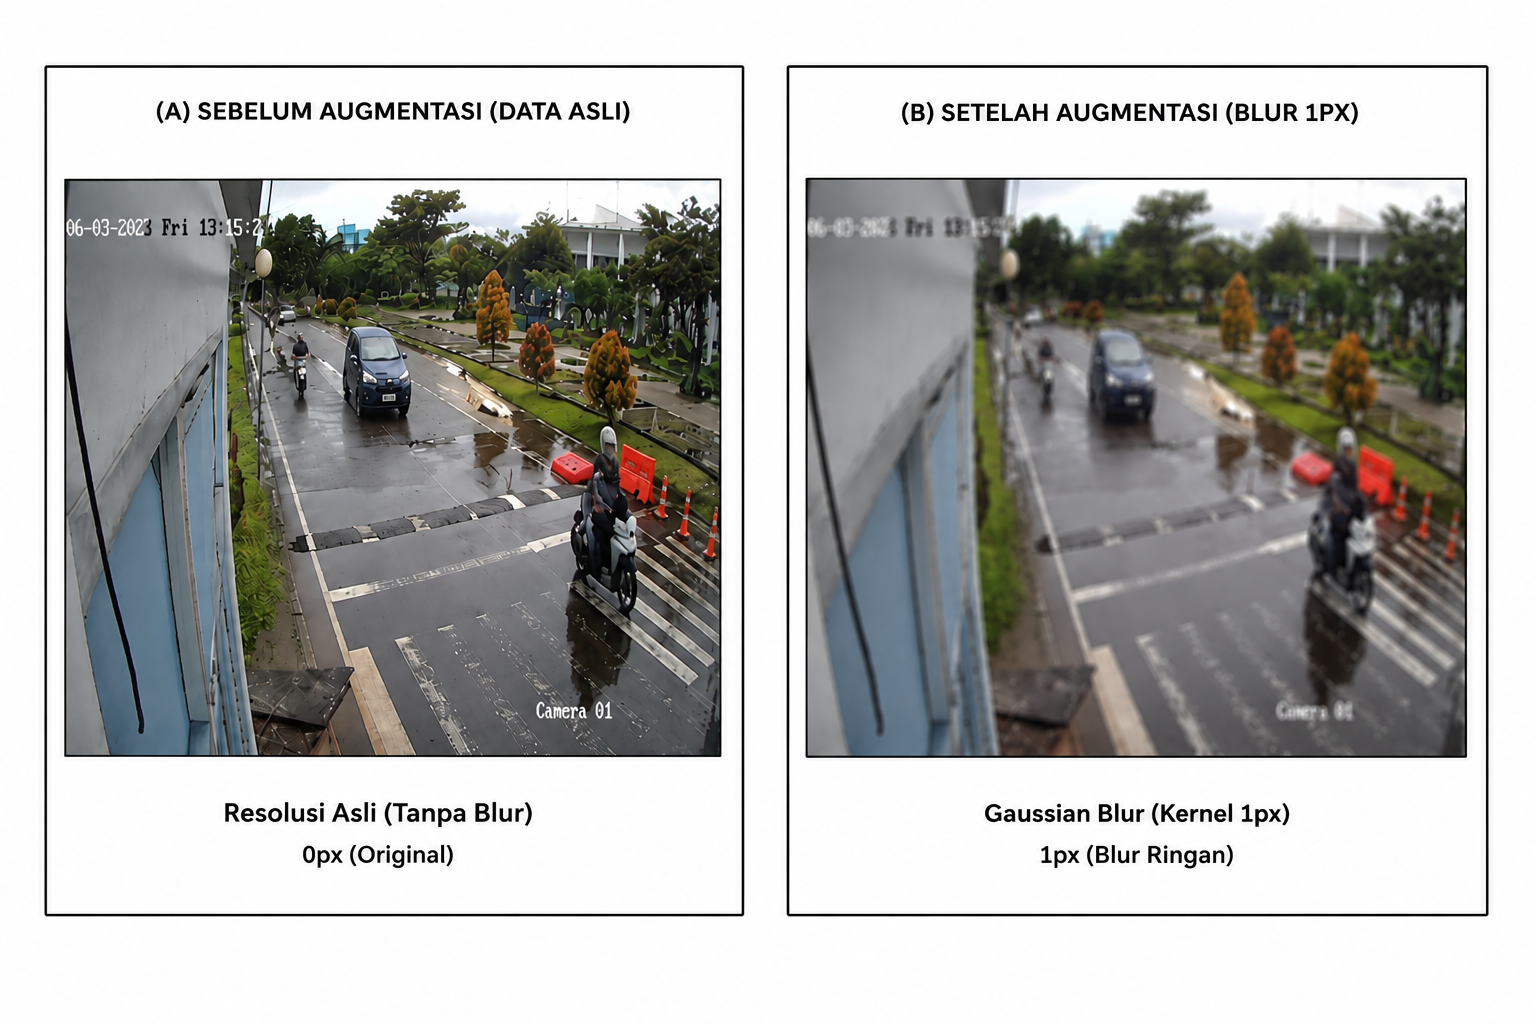
\includegraphics[width=0.95\textwidth]{gambar/aug_blur.jpg}
  \caption{Augmentasi \textit{Gaussian blur} dengan \textit{kernel} 1 piksel.}
  \label{fig:aug-blur}
\end{figure}

\textit{Gaussian blur} dengan \textit{kernel} 1 piksel meniru kondisi kamera CCTV yang sedikit kehilangan fokus, misalnya karena embun pada lensa atau udara berkabut. Citra hasil augmentasi terlihat sedikit kabur tetapi bentuk objek tetap dapat dibedakan. Pelatihan dengan citra kabur ini menahan model agar tidak bergantung pada ketajaman tepi saat melakukan deteksi.

\begin{figure}[H]
  \centering
  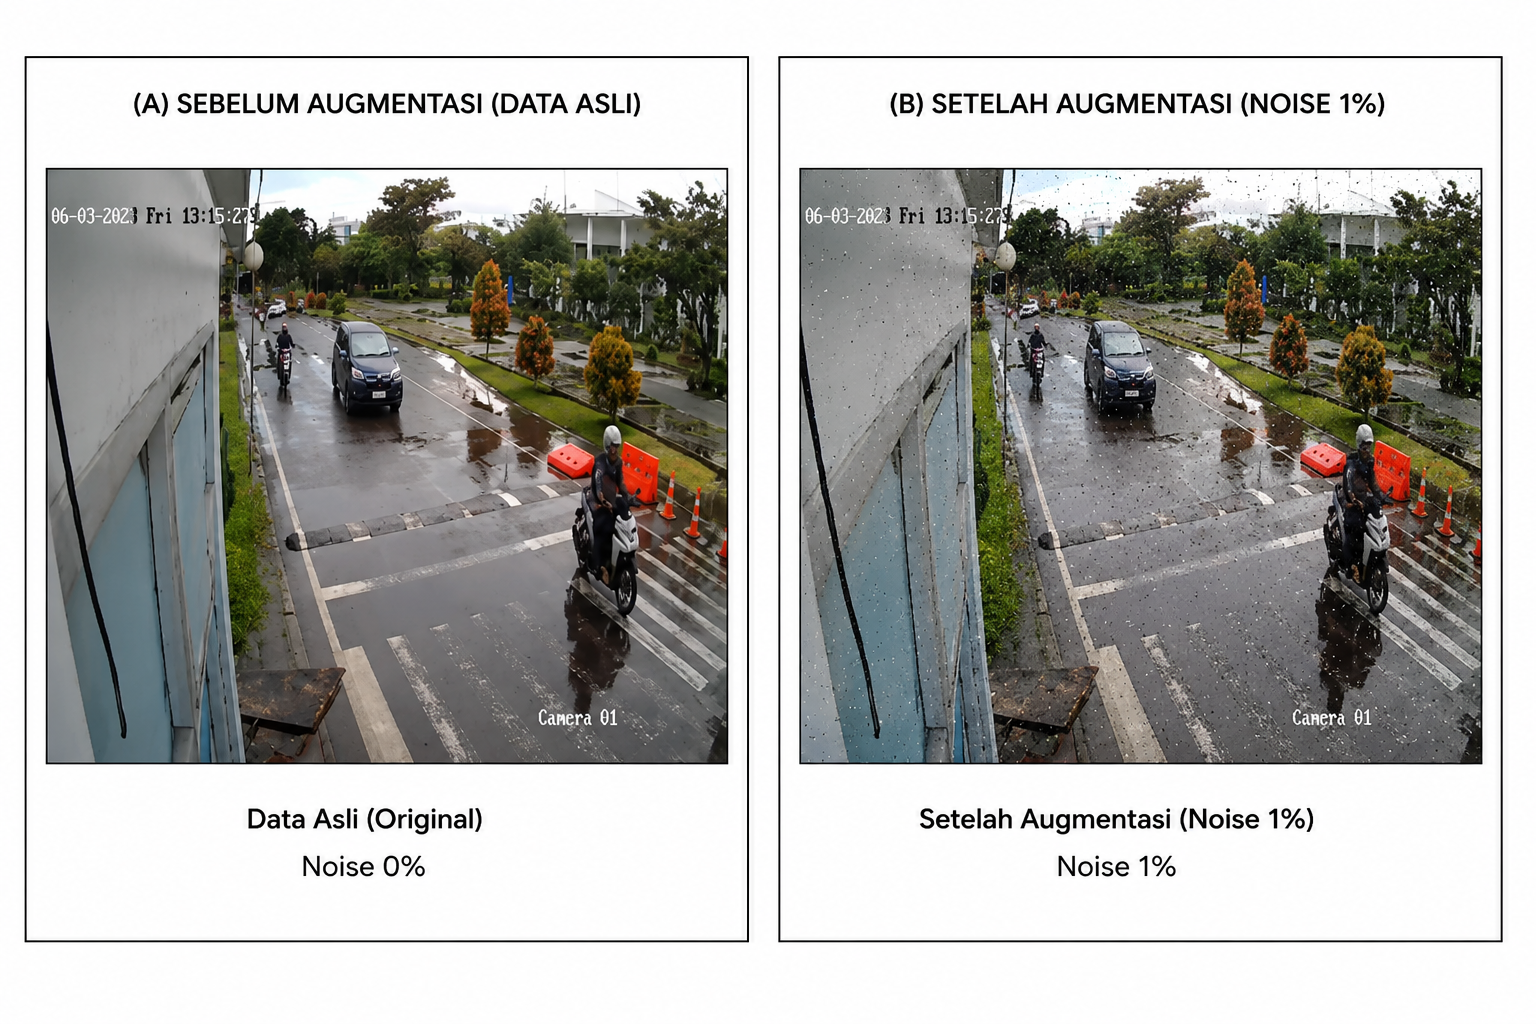
\includegraphics[width=0.8\textwidth]{gambar/aug_noise.jpg}
  \caption{Augmentasi \textit{additive noise} sebesar 1\% dari total piksel.}
  \label{fig:aug-noise}
\end{figure}

Penambahan \textit{additive noise} sebesar 1\% menirukan \textit{grain} sensor kamera pada kondisi cahaya rendah, kompresi \textit{streaming} yang agresif, atau interferensi sinyal pada CCTV analog. Bintik halus yang muncul mengaburkan detail tepi objek tanpa mengubah bentuk keseluruhan, sehingga model tetap dapat mengenali pengendara meskipun citra penuh artefak.

Kelima teknik di atas dilengkapi dengan \textit{motion blur} berpanjang 10 piksel yang meniru jejak gerak ketika kendaraan melintas cepat atau \textit{frame rate} CCTV menurun. Secara keseluruhan, kombinasi enam teknik tersebut menekan risiko \textit{overfitting} terhadap kondisi visual tertentu dan membantu model tetap mengenali objek meskipun kondisi citra di lapangan berbeda dari data pelatihan \cite{shorten2019survey}.

%
\subsection{Pemisahan Dataset dan Pelatihan Model}
\label{subsec:training-config}
%

Dataset yang sudah diperluas dibagi dengan rasio 82\% pelatihan (699 citra), 9\% validasi (79 citra), dan 9\% pengujian (78 citra). Pembagian ini memberi paparan data pelatihan yang cukup luas dan tetap menyisakan himpunan terpisah untuk memantau generalisasi selama optimasi. Pelatihan berjalan selama 300 \textit{epoch} pada layanan terkelola Roboflow Train 3.0 dengan varian \textit{Roboflow 3.0 Object Detection (Fast)} yang berbasis arsitektur YOLOv8n (lihat Sub-bab~\ref{subsec:pelatihan-yolov8n}). Proses pelatihan memantau tiga komponen galat: \textit{box loss} (kesalahan posisi dan ukuran \textit{bounding box}), \textit{class loss} (kesalahan klasifikasi kelas), dan \textit{distribution focal loss} atau DFL (kesalahan distribusi posisi tepi \textit{bounding box}). Kurva ditampilkan pada dua gambar terpisah agar dinamika pelatihan dan validasi dapat dibaca secara berdampingan: Gambar~\ref{fig:train-loss} memuat kurva pada data pelatihan, sedangkan Gambar~\ref{fig:val-loss} memuat kurva pada data validasi.

\begin{figure}[H]
\centering
\includegraphics[width=\textwidth]{gambar/train_los.jpg}
\caption{Dinamika \textit{train loss} model YOLOv8 selama 300 \textit{epoch}: (A) \texttt{train/box\_loss}, (B) \texttt{train/cls\_loss}, dan (C) \texttt{train/dfl\_loss}.}
\label{fig:train-loss}
\end{figure}

Gambar~\ref{fig:train-loss} menyajikan tiga kurva galat pada data pelatihan sepanjang 300 \textit{epoch}. Pada panel (A), \texttt{train/box\_loss} turun dari sekitar 2,0 di \textit{epoch} awal hingga sekitar 0,5 menjelang \textit{epoch} 300. penurunan paling tajam terjadi dalam 30 \textit{epoch} pertama ketika model mengkalibrasi ukuran dan posisi \textit{bounding box} pada kelas \texttt{MOTORCYCLE} yang dominan secara piksel. Setelah \textit{epoch} 50, kurva melandai dengan derau kecil, sebagai tanda posisi \textit{bounding box} semakin mantap dipelajari. Pada panel (B), \texttt{train/cls\_loss} jatuh tajam dari 4,0 ke sekitar 1,0 hanya dalam 10 \textit{epoch} pertama, lalu terus melandai sampai sekitar 0,4 di akhir pelatihan. Penurunan awal yang cepat ini selaras dengan perbedaan visual yang cukup tegas antara ketiga kelas, sehingga model cepat memetakan pemisahan kelas. Pada panel (C), \texttt{train/dfl\_loss} bergerak dari 1,55 menuju 0,83 dengan penurunan yang lebih landai dibanding dua kurva sebelumnya. Pola ini menunjukkan bahwa penajaman tepi \textit{bounding box} memang lebih lambat dipelajari, namun tetap konsisten menurun tanpa lonjakan sebagai indikator pelatihan yang stabil.

\begin{figure}[H]
\centering
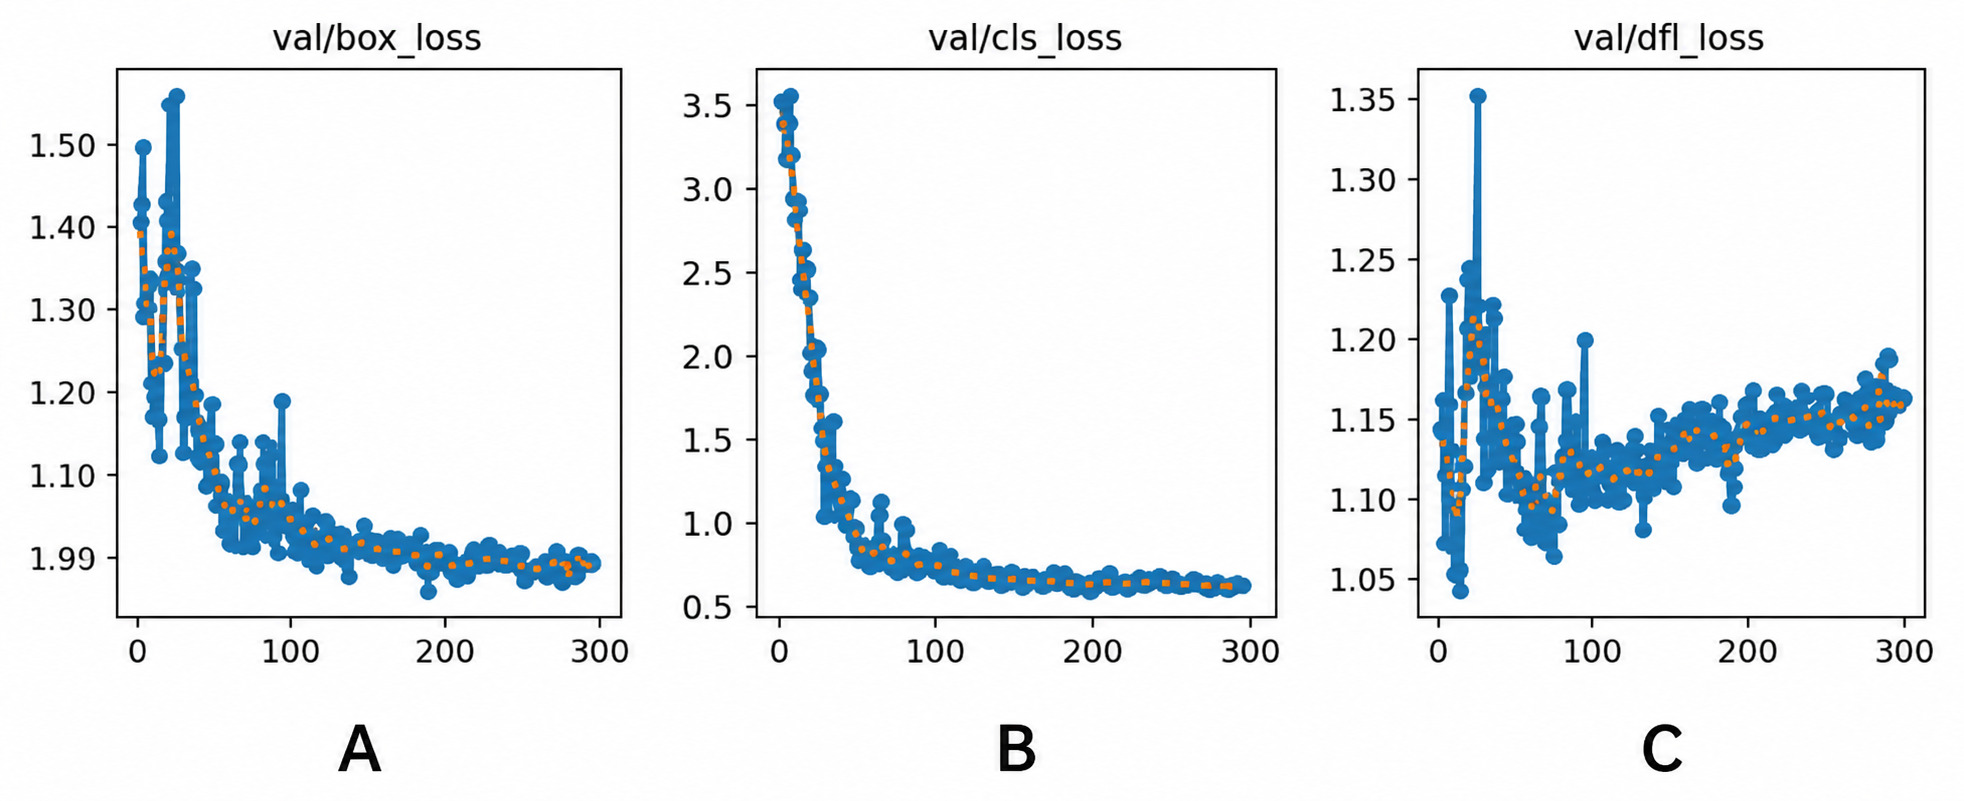
\includegraphics[width=\textwidth]{gambar/val_loss.jpg}
\caption{Dinamika \textit{validation loss} model YOLOv8 selama 300 \textit{epoch}: (A) \texttt{val/box\_loss}, (B) \texttt{val/cls\_loss}, dan (C) \texttt{val/dfl\_loss}.}
\label{fig:val-loss}
\end{figure}

Gambar~\ref{fig:val-loss} menyajikan tiga kurva galat pada data validasi yang dapat dibaca berdampingan dengan Gambar~\ref{fig:train-loss}. Pada panel (A), \texttt{val/box\_loss} dimulai pada kisaran 1,4--1,5 dan masih bergejolak pada 30--90 \textit{epoch} pertama dengan beberapa lonjakan ke atas 1,5. lonjakan ini muncul saat model mulai sensitif terhadap objek di luar pola dominan data pelatihan, misalnya tekstur latar yang menyerupai motor. Mulai \textit{epoch} 150, kurva mendatar di sekitar 0,99 dan bertahan sampai \textit{epoch} 300 tanpa kenaikan berarti, sebagai tanda lokalisasi \textit{bounding box} pada data validasi sudah konvergen. Panel (B) memperlihatkan \texttt{val/cls\_loss} dengan pola paling rapi: turun tajam dari 3,5 ke 1,0 sebelum \textit{epoch} 30, kemudian melandai sampai sekitar 0,6 di akhir pelatihan tanpa fluktuasi besar, sehingga klasifikasi kelas pada data validasi terbukti stabil. Pada panel (C), \texttt{val/dfl\_loss} sempat turun dari 1,15 ke kisaran 1,05--1,10 dalam 60 \textit{epoch} pertama, lalu merangkak naik perlahan ke kisaran 1,15--1,16 hingga \textit{epoch} 300. Kenaikan tipis ini umum terjadi pada DFL ketika model semakin tegas mengikuti distribusi tepi data pelatihan. selisihnya kecil dan tidak diiringi kenaikan pada \texttt{val/cls\_loss} maupun \texttt{val/box\_loss}, sehingga belum tergolong \textit{overfit}. Secara keseluruhan, kurva pelatihan menurun mulus dan kurva validasi mengikuti tren serupa dengan jarak yang masuk akal, sehingga 300 \textit{epoch} dinilai cukup untuk menghentikan pelatihan tanpa perlu \textit{early stopping} yang agresif.

\subsection{Evaluasi Kinerja Model}
\label{subsec:evaluasi-kinerja}
% ============================================================

Setelah pelatihan selesai, kinerja model dinilai pada himpunan validasi (\textit{validation set}) memakai tiga metrik: \textit{Mean Average Precision} pada ambang IoU 50\% (mAP@50), \textit{precision}, dan \textit{recall}. Ketiganya dipakai berbarengan karena \textit{precision} dan \textit{recall} menunjukkan keseimbangan antara deteksi yang benar dan yang terlewat, sedangkan mAP merangkum kualitas deteksi di berbagai ambang \textit{confidence} dalam satu angka. Ringkasannya ada pada Tabel~\ref{tab:metrik-validasi}.

%  EVIDENCE 1
\begin{table}[htbp]
\centering
\caption{Ringkasan metrik model YOLOv8 pada data validasi.}
\label{tab:metrik-validasi}
\begin{tabular}{lc}
\toprule
\textbf{Metrik} & \textbf{Nilai} \\
\midrule
\textit{Mean Average Precision} (mAP@50) & 91,4\% \\
\textit{Precision}  & 87,5\% \\
\textit{Recall}     & 86,5\% \\
\textit{F1 Score}     & 87.0\% \\
\bottomrule
\end{tabular}
\end{table}

%  ANALITIK 1
Tabel~\ref{tab:metrik-validasi} merangkum empat metrik utama model pada data validasi. \textit{Precision} 87,5\% dan \textit{recall} 86,5\% hanya berselisih 1,0 \%, yang berarti model tidak terlalu agresif hingga memunculkan banyak deteksi keliru, dan juga tidak terlalu hati-hati hingga melewatkan objek yang ada. Skor F1-nya rata-rata harmonik antara \textit{precision} dan \textit{recall} berada di kisaran 87,0\%, sehingga keseimbangan kedua metrik tersebut memang nyata dan bukan akibat salah satu sisi yang menutupi sisi lain. Pemakaian \textit{Region of Interest} (ROI) ikut menahan \textit{precision} tetap di atas 85\%. tanpa ROI, model akan menanggapi tekstur latar di trotoar dan jalur berlawanan, lalu memunculkan banyak \textit{false positive}. Pada skenario \textit{streaming} di gerbang Itera, \textit{precision} di atas 85\% perlu dijaga karena setiap deteksi yang keliru akan memicu pencatatan dan pengiriman notifikasi ke \textit{dashboard} yang sebenarnya tidak diperlukan.

Nilai mAP@50 sebesar 91,4\% setara dengan kinerja sistem deteksi pelanggaran helm berbasis YOLOv8 pada skenario waktu nyata yang dilaporkan oleh \cite{aboah2023helmet}. Sementara itu, \textit{precision} dan \textit{recall} yang masih di bawah 90\% menandakan model belum sepenuhnya rapi, terutama pada objek kecil dengan fitur yang serupa. Sumber kesalahan paling sering berasal dari perbedaan skala antara badan sepeda motor dan area pengendara: kepala hanya mengisi sebagian kecil piksel di citra, dan ketika motor menjauh dari kamera, detail visualnya semakin tipis. Pada kondisi tersebut, model lebih mudah salah membedakan pengendara berhelm, pengendara bertopi, atau pengendara berambut tebal. Catatan yang perlu disampaikan terbuka: \textit{recall} 86,5\% berarti sekitar 13,5\% pelanggaran lolos deteksi (\textit{false negatives}) di himpunan validasi angka yang masih dapat dipangkas lebih jauh oleh filter spasial IoA dan konfirmasi temporal \textit{N-frame} di tahap berikutnya pada \textit{pipeline}.

Kinerja model di luar data yang sudah dipelajari kemudian diuji pada data uji (\textit{test set}) yang terpisah sepenuhnya dari proses pelatihan. Hasil per kelas berupa \textit{Average Precision} (AP) pada ambang IoU 50\% ditampilkan pada Tabel~\ref{tab:metrik-test-objek}.

%  EVIDENCE 2
\begin{table}[htbp]
\centering
\caption{Nilai \textit{Average Precision} (AP@50) tiap kelas pada data uji.}
\label{tab:metrik-test-objek}
\begin{tabular}{lc}
\toprule
\textbf{Kategori Objek} & \textbf{AP@50} \\
\midrule
\texttt{Keseluruhan (All)}  & 90,0\% \\
\texttt{MOTORCYCLE}         & 94,0\% \\
\texttt{DRIVER\_NO\_HELMET} & 90,0\% \\
\texttt{DRIVER\_HELMET}     & 87,0\% \\
\bottomrule
\end{tabular}
\end{table}

%  ANALITIK 2
Tabel~\ref{tab:metrik-test-objek} menyajikan AP@50 tiap kelas beserta nilai agregat pada himpunan uji. Kinerja agregat di himpunan uji (mAP@50 = 90,0\%) hanya berbeda 1,4 \% dari himpunan validasi (mAP@50 = 91,4\%), sehingga model tidak \textit{overfit} pada data pelatihan dan masih dapat diandalkan ketika menghadapi citra baru. AP per kelas mengikuti pola yang sejalan dengan ukuran objek di citra: \texttt{MOTORCYCLE} memperoleh AP tertinggi 94,0\% karena badan motor mengisi piksel dominan dan bentuknya relatif konsisten dari satu citra ke citra lain, sedangkan dua kelas atribut kepala memperoleh AP lebih rendah. Selisih 7,0  antara \texttt{MOTORCYCLE} dan \texttt{DRIVER\_HELMET} menegaskan bahwa kesulitan utama model bukan saat mendeteksi objek besar, melainkan saat mengenali atribut kecil seperti helm. Pola yang sama soal \textit{scale imbalance} pada deteksi objek kecil dilaporkan pula oleh \cite{oksuz2020imbalance}.

Perbandingan dua kelas pelanggaran memperlihatkan pola. Model justru lebih presisi mendeteksi \texttt{DRIVER\_NO\_HELMET} (90,0\%) dibanding \texttt{DRIVER\_HELMET} (87,0\%), padahal jumlah anotasinya hampir sama (730 berbanding 718). Selisih 3,0 \% ini menandakan bahwa fitur visual ``tanpa helm'' siluet kepala terbuka, rambut, dan kulit lebih mudah dipelajari daripada variasi tampilan helm di lapangan. Helm yang muncul di area gerbang datang dalam berbagai bentuk, warna, dan ukuran, variasinya bertambah karena pantulan cahaya pagi atau sore kerap menutupi sebagian permukaan helm, dan kaca depan, penumpang, atau tas sering menghalangi sebagian helm. Akibatnya, fitur ``berhelm'' yang ditangkap model lebih bervariasi sehingga model lebih sering salah klasifikasi.  kelas yang paling krusial bagi sistem ini adalah \texttt{DRIVER\_NO\_HELMET}, dan kelas itulah yang memperoleh AP lebih tinggi, sehingga sasaran utama sistem menemukan pelanggaran tetap tertangani dengan baik.

Secara keseluruhan, mAP@50 sebesar 90,0\% pada himpunan uji menandakan modul YOLOv8 sudah cukup siap untuk dipasang ke \textit{pipeline} \textit{streaming} bersama ByteTrack di Itera.

\section{\textit{Pipeline Streaming} Deteksi Waktu Nyata}
\label{sec:integrasi-pipeline}
 Subbab ini menguraikan arsitektur hulu-ke-hilir (\textit{end-to-end}) yang memadukan deteksi YOLOv8 dan pelacakan multiobjek ByteTrack untuk menjaga persistensi identitas kendaraan. Pembahasan mencakup orkestrasi \textit{pipeline}, penerapan penyaring spasial (\textit{Intersection over Area}) dan temporal (N-\textit{frame}) untuk menekan deteksi palsu, serta evaluasi beban komputasi di simpul tepi (\textit{edge throughput} dan latensi).

% 
\subsection{Arsitektur dan Alur Transformasi Data}
\label{subsec:arsitektur-alur}

\textit{Pipeline} dirancang sebagai rangkaian fungsi yang mengubah bentuk data secara bertahap, dari piksel mentah menjadi catatan peristiwa yang siap disimpan. \textit{Frame} video CCTV yang awalnya berupa matriks BGR berdimensi $1280 \times 720 \times 3$ distandarkan ke $640 \times 640 \times 3$ lalu masuk ke YOLOv8 untuk memperoleh \textit{bounding box}, label kelas, dan skor \textit{confidence}. Hasilnya diteruskan ke ByteTrack supaya tiap objek memperoleh \texttt{Track ID} yang dipertahankan antar-\textit{frame}. Setelah identitas terpasang, filter IoA menilai relasi spasial antara \texttt{DRIVER\_NO\_HELMET} dan \texttt{MOTORCYCLE}, lalu konfirmasi N-\textit{frame} menahan keputusan pelanggaran sampai status terbukti konsisten. Tahap akhir mengemas data lolos validasi ke JSON dan mengirimkannya ke Kafka.

\begin{figure}[htbp]
\centering
\resizebox{\textwidth}{!}{%
\begin{tikzpicture}[
  node distance=0.6cm,
  stage/.style={
    rectangle, rounded corners=4pt, draw=black!70, fill=blue!8,
    minimum width=3.2cm, minimum height=2.6cm, align=center,
    font=\small
  },
  arrow/.style={-{Stealth[length=3mm]}, thick, draw=black!60},
  datalabel/.style={font=\scriptsize\ttfamily, text=black!70, align=center},
]

% Nodes
\node[stage] (input) {
  \textbf{Input Frame}\\[2pt]
  OpenCV
};

\node[stage, right=of input] (yolo) {
  \textbf{YOLOv8}\\[2pt]
  Ekstraksi fitur
};

\node[stage, right=of yolo] (bytrack) {
  \textbf{ByteTrack}\\[2pt]
  Pelacakan multiobjek
};

\node[stage, right=of bytrack] (assoc) {
  \textbf{Asosiasi}\\
  \textbf{spasial}\\[2pt]
  Filter IoA
};

\node[stage, right=of assoc] (violation) {
  \textbf{Logika temporal}\\[2pt]
  Konfirmasi\\
  N-\textit{frame}
};

\node[stage, right=of violation] (kafka) {
  \textbf{Kafka}\\
  \textbf{Producer}\\[2pt]
  Aliran peristiwa
};

% Arrows with data labels
\draw[arrow] (input) -- (yolo)
node[midway, above, datalabel] {}
node[midway, below, datalabel] {};

\draw[arrow] (yolo) -- (bytrack)
node[midway, above, datalabel] {}
node[midway, below, datalabel] {};

\draw[arrow] (bytrack) -- (assoc)
node[midway, above, datalabel] {}
node[midway, below, datalabel] {};

\draw[arrow] (assoc) -- (violation)
node[midway, above, datalabel] {}
node[midway, below, datalabel] {};

\draw[arrow] (violation) -- (kafka)
node[midway, above, datalabel] {}
node[midway, below, datalabel] {};

\end{tikzpicture}
}%
\caption{Alur transformasi data pada \textit{pipeline} pemrosesan tepi: dari piksel mentah hingga paket JSON.}
\label{fig:pipeline-flow}
\end{figure}

Pada tahap awal, OpenCV membaca \textit{frame} dari kamera dan menyalinnya menjadi numerik. \textit{Resize} ke $640 \times 640$ dilakukan supaya dimensi masukan tetap kelipatan \textit{stride} 32 YOLOv8, sehingga inferensi tidak menghasilkan \textit{padding} yang menggeser posisi \textit{bounding box}. Inferensi YOLOv8 dijalankan dengan ambang \textit{confidence} 0,25 dan \textit{NMS IoU} 0,7 sesuai konfigurasi yang ditetapkan di Bab 3 sehingga deteksi berkualitas rendah tersaring lebih awal sekaligus menghindari penghapusan kotak yang sebenarnya tidak tumpang tindih. Cuplikan keluaran inferensi pada \textit{frame} awal pengujian disajikan di Tabel~\ref{tab:output-yolo}. Empat deteksi  dua \texttt{MOTORCYCLE} dan dua \texttt{DRIVER\_HELMET}  terbaca dengan \textit{confidence} 0,884 hingga 0,940 yang sudah cukup tinggi untuk diteruskan ke tahap pelacakan. Yang penting di tahap ini, ukuran data ringkas: tiap deteksi berbobot sekitar 40--60 \textit{byte} dibandingkan \textit{frame} mentah yang berbobot \textit{megabyte}, sehingga ukuran pada lapisan berikutnya tetap kecil.

\begin{table}[htbp]
\centering
\caption{Cuplikan keluaran inferensi YOLOv8 pada \textit{frame} awal pengujian.}
\label{tab:output-yolo}
\footnotesize
\setlength{\tabcolsep}{3pt}
\begin{tabular}{p{1.4cm} p{3.2cm} c c c c c}
\toprule
\textbf{No.} & \textbf{Kategori Objek} & \textbf{X1} & \textbf{Y1} & \textbf{X2} & \textbf{Y2} & \textbf{Confidence} \\
\midrule
1 & \texttt{MOTORCYCLE}      & 936{,}9  & 374{,}5 & 1061{,}2 & 526{,}2 & 0{,}9398 \\
2 & \texttt{MOTORCYCLE}      & 752{,}5  & 274{,}9 &  828{,}1 & 366{,}3 & 0{,}9262 \\
3 & \texttt{DRIVER\_HELMET}  & 767{,}4  & 227{,}4 &  812{,}6 & 341{,}0 & 0{,}8910 \\
4 & \texttt{DRIVER\_HELMET}  & 970{,}8  & 303{,}9 & 1037{,}8 & 480{,}2 & 0{,}8840 \\
\bottomrule
\end{tabular}
\end{table}

ByteTrack menerima keluaran YOLOv8 lalu memberi \texttt{Track ID} kepada tiap objek. Begitu identitas terpasang, sistem menghitung IoA antara setiap kandidat pengendara dan motor terdekat untuk menilai apakah relasi spasial keduanya sah sebagai aksi berkendara. Tabel~\ref{tab:output-bytetrack-ioa} memperlihatkan, pada \textit{frame} yang sama, dua \texttt{DRIVER\_HELMET} memperoleh IoA 0,582 dan 0,600 terhadap \texttt{MOTORCYCLE} pasangannya  keduanya jelas di atas ambang 0,3. Pasangan tersebut artinya Track 3 sangat berdekatan hingga bisa diasumsikan bahwa \texttt{DRIVER\_HELMET} Track 3 mengendari \texttt{MOTORCYCLE} Track 1. Tahap berikutnya, yaitu konfirmasi temporal N-\textit{frame}, baru relevan ketika kelas yang dilacak adalah \texttt{DRIVER\_NO\_HELMET}. Status pelanggaran tidak langsung dicatat saat satu \textit{frame} terbaca tanpa helm. sistem menahannya sampai status sama bertahan minimal tiga \textit{frame} berturut-turut. Mekanisme penundaan ini digambarkan di Gambar~\ref{fig:streak-timeline}: nilai \textit{streak} naik dari 1, 2, lalu 3, dan \textit{event} baru dilepas setelah ambang $N=3$ tercapai. Dengan cara itu, kilatan deteksi sesaat akibat bayangan atau pantulan tidak ikut tercatat sebagai pelanggaran. Sebaliknya, ketika deteksi sesaat menghilang akibat oklusi parsial, mekanisme \textit{patience-based decay} membiarkan \textit{streak} tetap aktif selama lima \textit{frame} tambahan sebelum dihapus, sehingga akumulasi pelanggaran yang sedang berjalan tidak gugur hanya karena satu \textit{frame} terhalang sesaat.

\begin{table}[htbp]
\centering
\caption{Cuplikan keluaran ByteTrack dan nilai IoA pada \textit{frame} awal.}
\label{tab:output-bytetrack-ioa}
\small
\resizebox{\textwidth}{!}{%
\begin{tabular}{cclcc}
\toprule
\textbf{Track ID} & \textbf{Kategori Objek} & \textbf{Pasangan} & \textbf{Nilai IoA} & \textbf{Hasil} \\
\midrule
1 & \texttt{MOTORCYCLE}      & - & - & Kendaraan (\textit{carrier}) \\
2 & \texttt{MOTORCYCLE}      & - & - & Kendaraan (\textit{carrier}) \\
3 & \texttt{DRIVER\_HELMET}  & Berpasangan dengan ID 2 & 0{,}5820 & Valid (\checkmark) \\
4 & \texttt{DRIVER\_HELMET}  & Berpasangan dengan ID 1 & 0{,}5996 & Valid (\checkmark) \\
\bottomrule
\end{tabular}
}
\end{table}

\begin{figure}[htbp]
\centering
\begin{tikzpicture}[
frame/.style={rectangle, draw, minimum width=1.1cm, minimum height=0.7cm,
font=\small, align=center},
confirmed/.style={frame, fill=red!20},
streak/.style={frame, fill=yellow!20},
normal/.style={frame, fill=green!10},
]

% Timeline
\node[normal] (f1) at (0,0) {Frame 1\\streak=1};
\node[streak] (f2) at (2.2,0) {Frame 2\\streak=2};
\node[confirmed] (f3) at (4.4,0) {Frame 3\\streak=3};

% Labels
\node[above=0.3cm of f1, font=\scriptsize] {NO\_HELMET};
\node[above=0.3cm of f2, font=\scriptsize] {NO\_HELMET};
\node[above=0.3cm of f3, font=\scriptsize] {NO\_HELMET};

% Arrow
\draw[-{Stealth}, thick] (f1) -- (f2);
\draw[-{Stealth}, thick] (f2) -- (f3);

% Confirmation marker
\node[below=0.4cm of f3, font=\small\bfseries, text=red!70!black] {%
Ambang $N=3$ Tercapai $\Rightarrow$ Kirim Event
};

% Track ID label
\node[left=0.5cm of f1, font=\small] {\textbf{Track ID = 4:}};

\end{tikzpicture}
\caption{\textit{Timeline} konfirmasi temporal: pelanggaran tercatat hanya setelah objek \texttt{DRIVER\_NO\_HELMET} bertahan minimal tiga \textit{frame} berturut-turut.}
\label{fig:streak-timeline}
\end{figure}

Setelah lolos dua filter, sistem membungkus informasi pelanggaran ke dalam paket JSON sebelum melepasnya ke Kafka. Tabel~\ref{tab:json-output} menampilkan struktur paketnya. Beberapa \textit{field} dipasang dengan sengaja untuk kebutuhan hulu-ke-hilir: \texttt{event\_id} berupa UUID menjamin setiap kejadian unik secara global, \texttt{timestamp} berpresisi tinggi memungkinkan dimensi waktu dibangun di \textit{data mart}, sedangkan \texttt{track\_id} memberi penanda untuk \textit{dedup} di Spark. Nilai pada \textit{field} \texttt{confidence} diisi dengan rata-rata \textit{confidence} sepanjang $N$ \textit{frame} yang membentuk \textit{streak} pelanggaran, bukan \textit{confidence} \textit{frame} terakhir, agar angka yang tercatat lebih merepresentasikan keseluruhan periode pelanggaran. \textit{Field} \texttt{bbox} dan \texttt{latency\_ms} tidak wajib dipakai \textit{dashboard}, tetapi dipertahankan untuk keperluan audit dan analisis kinerja. Ukuran satu pesan berkisar 335 \textit{byte}, jadi jalur Kafka tetap ringan walaupun trafik kampus melonjak. Contoh keluaran di atas memperlihatkan tiap tahap berjalan benar pada \textit{frame} awal.

\begin{table}[htbp]
\centering
\caption{Struktur paket data JSON yang dikirim ke Kafka.}
\label{tab:json-output}
\footnotesize
\setlength{\tabcolsep}{4pt}
\begin{tabular}{p{0.18\textwidth} p{0.24\textwidth} p{0.46\textwidth}}
\toprule
\textbf{Field} & \textbf{Contoh Nilai} & \textbf{Keterangan} \\
\midrule
\texttt{event\_id}     & \texttt{"b11c5428-0c99..."}    & UUID unik tiap kejadian \\
\texttt{track\_id}     & \texttt{15}                    & Identitas objek dari ByteTrack \\
\texttt{timestamp}     & \texttt{"2026-03-03T20:41..."} & Waktu kejadian \\
\texttt{camera\_id}    & \texttt{"gate\_utama\_01"}     & Lokasi sumber deteksi \\
\texttt{violation\_type} & \texttt{"no\_helmet"}         & Jenis pelanggaran \\
\texttt{confidence}    & \texttt{0.8939}                & Tingkat keyakinan model YOLO \\
\texttt{bbox\_[xy12]}  & \texttt{990, 312, 1058, 490}   & Koordinat \textit{bounding box} \\
\texttt{frame\_number} & \texttt{3}                     & Posisi \textit{frame} dalam aliran video \\
\texttt{latency\_ms}   & \texttt{58.94}                 & Latensi pemrosesan \textit{frame} \\
\bottomrule
\end{tabular}
\end{table}

% 
\subsection{Persistensi Identitas dan Filter Spasial-Temporal}
\label{subsec:persistensi-filter}

Setelah \textit{pipeline} terbukti berjalan benar pada \textit{frame} awal, pengujian diperluas ke 3.001 \textit{frame} video gerbang utama Itera yang merekam lalu lintas pada jam aktif. Dua hal yang paling menentukan kelayakan sistem diuji bersamaan, yaitu kemampuan ByteTrack menjaga identitas tiap objek selama mungkin dan kekuatan filter berlapis menyaring deteksi mentah agar yang tersisa hanya \textit{event} yang layak dicatat. Pembahasan di bagian ini menyusur kedua aspek tersebut secara berurutan.

Pelacakan ByteTrack pada keseluruhan \textit{frame} dirangkum di Tabel~\ref{tab:bytetrack-basic-stats}. Sistem mencatat 134 objek unik dengan rata-rata 3,36 objek aktif per \textit{frame} dan puncak 11 objek pada momen padat. Durasi pelacakan terpanjang menyentuh 419 \textit{frame}, setara sekitar 22 detik pada laju efektif \textit{pipeline} 18,9 FPS. Angka-angka ini cocok dengan kondisi gerbang kampus: kepadatan biasanya muncul pada pergantian jam kuliah, dan ByteTrack masih sanggup melayani belasan objek tanpa kehilangan identitas. Ada satu catatan yang perlu disampaikan terbuka: \texttt{Track ID} di sini adalah identitas sesi pelacakan, bukan identitas pelanggar yang permanen. Saat objek menghilang dari pandangan lebih lama dari \textit{lost track buffer} 60 \textit{frame}, ByteTrack memberi ID baru begitu objek muncul kembali. Akibatnya, satu pengendara yang masuk-keluar area pantau beberapa kali bisa terhitung sebagai entitas berbeda. Batasan ini melekat pada pelacak tanpa modul \textit{re-identification} dan dimasukkan ke agenda pengembangan lanjut \cite{zhang2022bytetrack_eccv}.

\begin{table}[htbp]
\centering
\caption{Statistik pelacakan ByteTrack pada 3.001 \textit{frame} video uji.}
\label{tab:bytetrack-basic-stats}
\begin{tabular}{lc}
\toprule
\textbf{Parameter} & \textbf{Nilai} \\
\midrule
Jumlah objek unik terlacak & 134 objek \\
Rata-rata objek aktif per \textit{frame} & 3,36 objek \\
Puncak objek bersamaan dalam satu \textit{frame} & 11 objek \\
Durasi pelacakan terpanjang & 419 \textit{frame} \\
\bottomrule
\end{tabular}
\end{table}

Ketahanan pelacakan diuji lebih jauh pada situasi oklusi, yaitu saat objek sempat tertutup kendaraan lain selama beberapa \textit{frame}. Gambar~\ref{fig:occlusion-handling} memperlihatkan satu pengendara yang hilang di balik mobil, lalu kembali muncul dengan \texttt{Track ID} yang sama. Dua mekanisme bekerja di balik kestabilan ini. Pertama, ByteTrack memakai asosiasi dua tahap: deteksi \textit{confidence} tinggi disambung ke trek aktif terlebih dahulu, lalu deteksi \textit{confidence} rendah dipakai untuk menyambung trek yang sempat terputus \cite{ma2023adaptivebytetrack}. Kedua, \textit{lost track buffer} 60 \textit{frame} menahan trek tidak langsung dihapus saat halangan datang. Kombinasi keduanya memastikan pencatatan pelanggaran tidak terputus akibat oklusi sesaat yang lazim ditemui di lalu lintas nyata.

\begin{figure}[H]
\centering
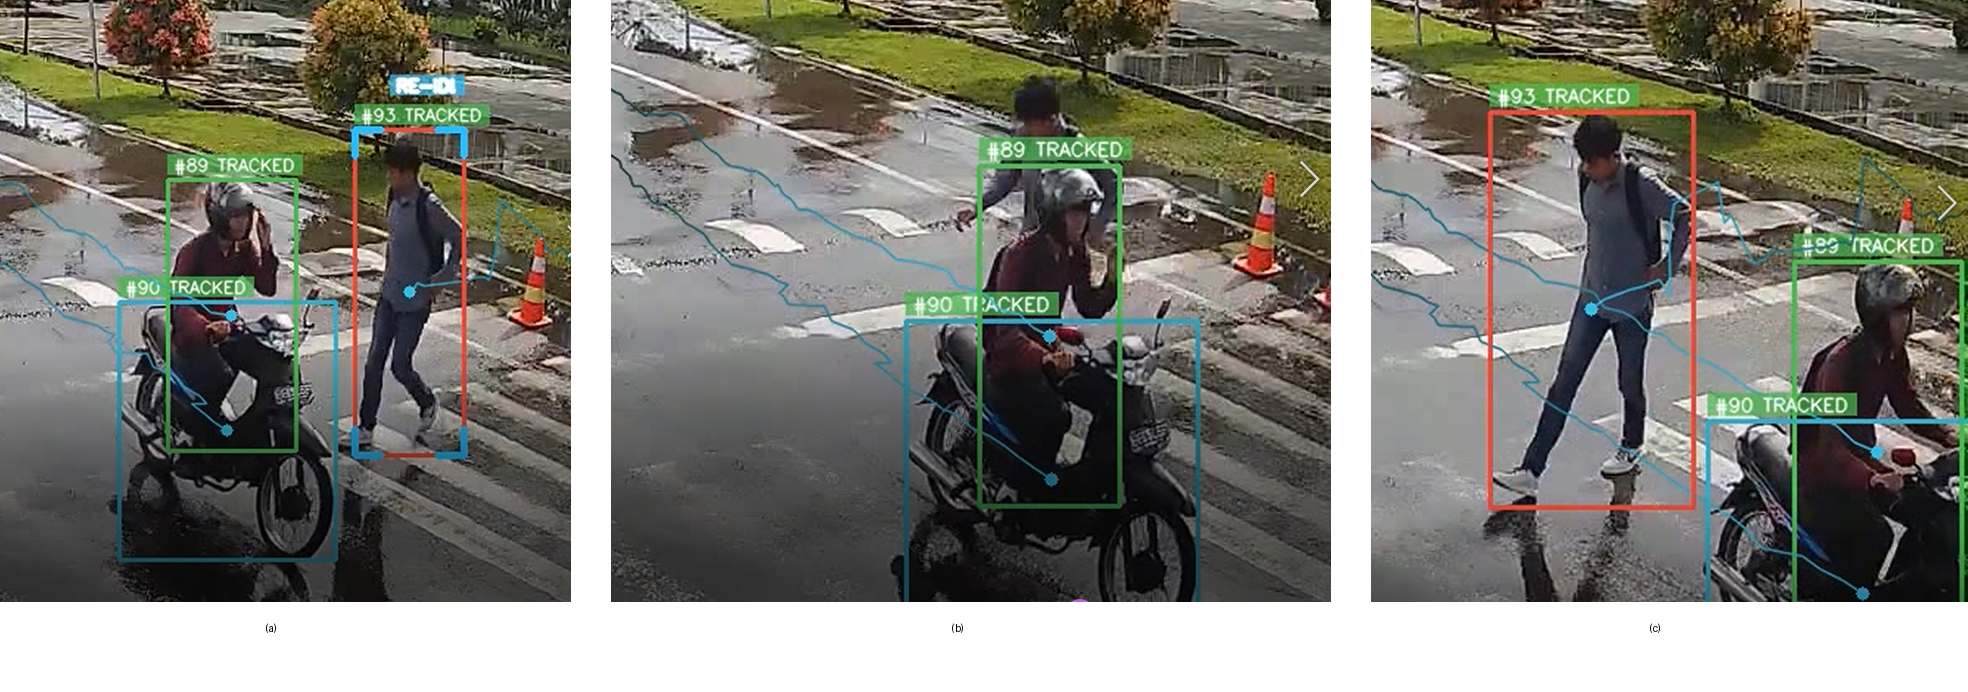
\includegraphics[width=0.95\textwidth]{gambar/figure_sequence_abc.png}
\caption{Ketahanan pelacakan ByteTrack saat oklusi: \texttt{Track ID} tetap melekat meski objek sempat tertutup kendaraan lain.}
\label{fig:occlusion-handling}
\end{figure}

Tabel~\ref{tab:filtering-funnel} merangkum selektivitas filter berlapis pada potongan uji 3.001 \textit{frame}. Tabel menampilkan lima metrik per tahap: nomor tahap, proses yang dijalankan, jumlah kandidat yang lolos, jumlah yang dibuang, dan persentase sisa terhadap deteksi mentah. Secara umum, jumlah kandidat turun monoton dari 9.544 di Tahap 0 hingga hanya 2 \textit{event} unik di Tahap 5---reduksi sekitar 800 kali. Penurunan paling tajam terjadi di Tahap 3 (IoA spasial) yang sekali jalan membuang 97,8\% kandidat, sementara Tahap 2 (\textit{Track ID}) sengaja tidak mereduksi data karena perannya menyiapkan fondasi identitas bagi tahap berikutnya. Pembahasan tahap demi tahap dipaparkan setelah tabel.

\begin{table}[htbp]
\centering
\caption{Reduksi jumlah deteksi tiap tahap filter pada 3.001 \textit{frame}.}
\label{tab:filtering-funnel}
\small
\setlength{\tabcolsep}{2pt}
\scriptsize
\begin{tabular}{p{1.2cm}p{2.0cm}p{2.0cm}p{2.0cm}p{2.0cm}}
\toprule
\textbf{Tahap} & \textbf{Proses} & \textbf{Jumlah} & \textbf{Dibuang} & \textbf{\% Sisa} \\
\midrule
0 & Deteksi mentah YOLO (semua kelas) & 9.544 &  & 100,0\% \\
1 & Ambil kelas \texttt{NO\_HELMET} & 1.602 & 7.942 & 16,8\% \\
2 & Pasang \textit{Track ID} & 1.602 & 0 & 16,8\% \\
3 & Filter spasial IoA ($\geq$0,3 ke motor) & 35 & 1.567 & 0,37\% \\
4 & Konfirmasi N-\textit{frame} ($\geq$3 \textit{frame}) & 25 & 10 & 0,26\% \\
5 & \textit{Dedup} per-\textit{track} (\textit{event} unik) & \textbf{2} & 23 & \textbf{0,02\%} \\
\bottomrule
\end{tabular}
\end{table}

Titik masuk seluruh \textit{pipeline} adalah keluaran mentah detektor YOLO yang pada potongan uji ini menghasilkan 9.544 \textit{bounding box} dari ketiga kelas, atau rata-rata 3,18 deteksi per \textit{frame} sejalan dengan rata-rata 3,36 objek aktif pada Tabel~\ref{tab:bytetrack-basic-stats}. Komposisi deteksi mentah didominasi \texttt{MOTORCYCLE} karena badan motor terlihat utuh di hampir setiap \textit{frame}, sedangkan \texttt{DRIVER\_HELMET} dan \texttt{DRIVER\_NO\_HELMET} muncul hanya saat kepala pengendara tidak terhalang penumpang atau kaca depan. Angka 9.544 ini sekaligus menjadi tolok ukur beban inferensi YOLOv8 dan pembagi untuk seluruh persentase di kolom \textit{\% Sisa}. Tanpa filter di tahap berikutnya, jumlah tersebut setara dengan ratusan ribu baris log per jam jika diekstrapolasi ke operasi penuh kamera gerbang.

Dari 9.544 deteksi mentah itu, filter \textit{class-conditional} pertama kali memangkas 7.942 deteksi non-target dan menyisakan 1.602 kandidat \texttt{DRIVER\_NO\_HELMET} atau 16,8\% dari mentah. Reduksi 83,2\% ini dicapai tanpa biaya komputasi berarti karena hanya membaca label keluaran YOLO, jauh lebih murah dibandingkan operasi geometris pada tahap-tahap berikutnya. Tujuan seleksi kelas ini bukan menyensor data lain, melainkan memfokuskan jalur pelanggaran: \texttt{MOTORCYCLE} tetap dilestarikan di tahap pelacakan untuk dipakai sebagai pasangan IoA di Tahap 3, sedangkan \texttt{DRIVER\_HELMET} memang tidak masuk jalur \textit{event}. Posisi filter ini di paling depan dirancang sengaja agar tahap mahal seperti IoA dan konfirmasi temporal hanya menghitung kandidat yang berpotensi menjadi pelanggaran.

Setelah kelas disaring, 1.602 kandidat tersebut diteruskan ke ByteTrack untuk disemati \textit{Track ID} persisten. Jumlah kandidat tidak berubah pada tahap ini (1.602 masuk, 1.602 keluar), namun keluaran ByteTrack mengubah karakter datanya: tiap kandidat kini membawa identitas yang konsisten lintas \textit{frame}, sehingga dua tahap berikutnya dapat berbicara tentang ``objek yang sama'' pada waktu yang berbeda dan bukan sekadar kotak deteksi anonim. Beban tambahan di sini terukur 1,62 milidetik per \textit{frame} pada Tabel~\ref{tab:latency-decomposition} atau hanya 3,1\% dari total latensi sistem harga yang sebanding dengan fungsinya sebagai fondasi konfirmasi N-\textit{frame} dan \textit{dedup}. Catatan yang perlu disampaikan terbuka: \texttt{Track ID} di sini bersifat identitas sesi pelacakan, bukan identitas pelanggar fisik permanen, sehingga pengendara yang masuk-keluar area pantau lebih dari 60 \textit{frame} akan memperoleh ID baru \cite{zhang2022bytetrack_eccv}.

Dengan identitas pelacakan yang sudah terpasang, filter spasial IoA kemudian menjadi penyaring paling agresif dengan membuang 1.567 dari 1.602 kandidat atau 97,8\% dalam satu langkah dan hanya meloloskan 35 kandidat. IoA yang dihitung mengikuti definisi pada Bab~\ref{chap:metodologi} membandingkan luas irisan \textit{bounding box} \texttt{DRIVER\_NO\_HELMET} terhadap luasnya sendiri, lalu menerima kandidat hanya bila skornya $\geq$0{,}3 terhadap salah satu \texttt{MOTORCYCLE} aktif. Mayoritas kandidat yang gugur berasal dari tiga sumber yang konsisten dengan kondisi gerbang Itera: pejalan kaki di sisi trotoar yang sesaat terklasifikasi sebagai \texttt{DRIVER\_NO\_HELMET}, \textit{false positive} di tepi citra yang tidak mempunyai pasangan motor, dan pengendara yang motornya sempat terhalang kendaraan lain sehingga relasi spasialnya tidak terbentuk. Pemilihan ambang 0{,}3 merupakan kompromi yang berhasil: nilai lebih rendah (0{,}1) akan meloloskan asosiasi palsu pada keramaian, sedangkan nilai lebih tinggi (0{,}5) akan menggugurkan kasus motor parsial yang sebenarnya valid. IoA dipilih ketimbang IoU karena \textit{bounding box} pengendara jauh lebih kecil daripada motor, sehingga IoU menghasilkan skor rendah meski pengendara jelas berada di atas motor.

Dari 35 kandidat yang lolos IoA, filter temporal kemudian membuang 10 di antaranya atau 28,6\% dari jumlah yang masuk, dan meneruskan 25 kandidat ke tahap berikutnya. Mekanismenya sederhana: \textit{streak} hanya naik bila status \texttt{DRIVER\_NO\_HELMET} bertahan pada \texttt{Track ID} yang sama di tiga \textit{frame} berturut-turut, sehingga deteksi yang berkedip akibat bayangan, pantulan kaca, atau klasifikasi salah sesaat tidak meneruskan langkah berikutnya. Filter ini menambah jeda pelaporan sekitar 150 milidetik (tiga \textit{frame} pada 18,9 FPS), nilai yang tetap nyaman untuk pemantauan \textit{near real-time} karena masih jauh di bawah ambang persepsi operator. Mekanisme \textit{patience-based decay} dengan lima \textit{frame} masa tenggang melengkapi filter ini agar \textit{streak} tidak gugur hanya karena oklusi sesaat oleh kendaraan lain sebuah kompromi praktis antara ketegasan dan ketahanan terhadap gangguan visual. Reduksi 28,6\% di sini relatif kecil dibanding Tahap 3, dan justru itu yang diharapkan: kandidat yang sudah lolos IoA umumnya merupakan pengendara nyata, sehingga filter temporal hanya memangkas sisa-sisa \textit{false positive} yang masih terbawa.

Tahap terakhir memadatkan 25 konfirmasi tingkat-\textit{frame} menjadi 2 \textit{event} unik dengan membuang 23 duplikat atau 92,0\% dari masukan. Logikanya, satu \texttt{Track ID} yang sudah melewati konfirmasi N-\textit{frame} bisa terus terkonfirmasi sepanjang pengendara terlihat di kamera, sehingga tanpa \textit{dedup}, satu orang yang melintas selama 5 detik pada 15 FPS dapat tercatat hingga 75 kali. \textit{Dedup} memakai \texttt{Track ID} sebagai kunci dan memilih konfirmasi pertama sebagai representasi \textit{event}, lalu menahan ID tersebut hingga sesi pelacakan berakhir. Implikasinya langsung terasa pada beban hilir: \textit{data mart} hanya menerima entri yang berkorelasi dengan pengendara unik, dan \textit{dashboard} menampilkan jumlah pelanggar bukan jumlah \textit{frame}. Keterbatasan tahap ini terikat pada keterbatasan penyematan ID di Tahap 2: ketika ByteTrack memberi ID baru karena objek menghilang lebih dari 60 \textit{frame}, pengendara yang sama dapat tercatat dua kali isu yang dimasukkan ke agenda \textit{re-identification} antarkamera.
% 
\subsection{Kinerja Sisi Tepi dan Distribusi Aliran}
\label{subsec:kinerja-edge-distribusi}


Gambar~\ref{fig:fps-timeseries-evidence} memperlihatkan dinamika \textit{throughput} \textit{pipeline} sepanjang 3.001 \textit{frame}. Rerata \textit{throughput} menyentuh 18,9 FPS dengan pola yang relatif rata sejak awal sampai akhir pengujian. Tidak ada tren penurunan yang berarti, jadi tidak ada indikasi kebocoran memori atau akumulasi beban yang membebani CPU seiring waktu. Dibandingkan kebutuhan CCTV kampus yang umumnya beroperasi pada 10 sampai 15 FPS, capaian 18,9 FPS menyisakan margin yang nyaman untuk menampung lonjakan kepadatan tanpa mengorbankan ketepatan waktu pencatatan.

\begin{figure}[htbp]
\centering
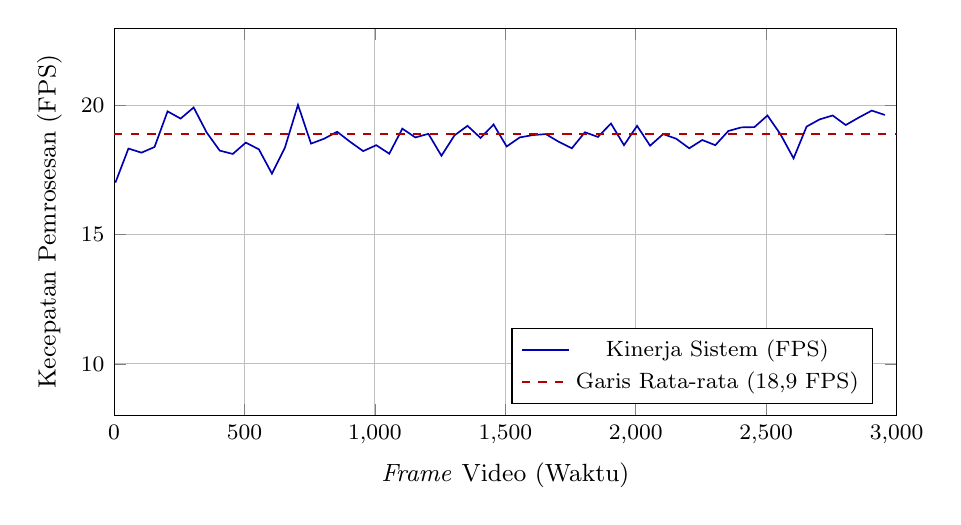
\begin{tikzpicture}
\begin{axis}[
  width=0.95\textwidth,
  height=6.5cm,
  xlabel={\textit{Frame} Video (Waktu)},
  ylabel={Kecepatan Pemrosesan (FPS)},
  xmin=0, xmax=3000,
  ymin=8, ymax=23,
  grid=major,
  grid style={line width=0.2pt, draw=gray!30},
  major grid style={line width=0.4pt, draw=gray!50},
  legend pos=south east,
  legend style={font=\footnotesize},
  tick label style={font=\footnotesize},
  label style={font=\small},
  title style={font=\small\bfseries},
]
% FPS time series (sampled every ~100 frames)
\addplot[blue!70!black, line width=0.6pt, mark=none] coordinates {
  (5,17.02) (55,18.34) (105,18.18) (155,18.40) (205,19.78)
  (255,19.50) (305,19.93) (355,18.96) (405,18.26) (455,18.13)
  (505,18.57) (555,18.31) (605,17.37) (655,18.38) (705,20.03)
  (755,18.53) (805,18.72) (855,18.99) (905,18.60) (955,18.24)
  (1005,18.47) (1055,18.14) (1105,19.11) (1155,18.77) (1205,18.91)
  (1255,18.06) (1305,18.85) (1355,19.22) (1405,18.75) (1455,19.27)
  (1505,18.42) (1555,18.77) (1605,18.86) (1655,18.90) (1705,18.60)
  (1755,18.35) (1805,18.97) (1855,18.79) (1905,19.31) (1955,18.47)
  (2005,19.22) (2055,18.45) (2105,18.90) (2155,18.72) (2205,18.35)
  (2255,18.67) (2305,18.47) (2355,19.02) (2405,19.16) (2455,19.17)
  (2505,19.62) (2555,18.89) (2605,17.96) (2655,19.19) (2705,19.47)
  (2755,19.62) (2805,19.25) (2855,19.54) (2905,19.81) (2955,19.64)
};
\addlegendentry{Kinerja Sistem (FPS)}
% Mean line
\addplot[red!70!black, dashed, line width=1pt, domain=0:3000] {18.9};
\addlegendentry{Garis Rata-rata (18,9 FPS)}
\end{axis}
\end{tikzpicture}
\caption{Dinamika \textit{throughput} \textit{pipeline} \textit{end-to-end}: rerata 18,9 FPS tanpa tren penurunan sepanjang pengujian.}
\label{fig:fps-timeseries-evidence}
\end{figure}

Tabel~\ref{tab:latency-decomposition} merinci dari mana 53 milidetik latensi per \textit{frame} itu berasal. Inferensi YOLOv8 mengambil porsi terbesar, yaitu 51,4 milidetik atau 96,8\% dari total. ByteTrack menambah 1,62 milidetik (3,1\%) dan seluruh modul \textit{filtering} hanya 0,05 milidetik (0,1\%). Penambahan logika pelacakan dan validasi spasial-temporal hampir tidak terasa di latensi, sehingga optimasi inferensi YOLOv8 berarti optimasi \textit{pipeline} secara keseluruhan \cite{zhang2022bytetrack_eccv}. Latensi total 53 milidetik tergolong responsif untuk pemantauan \textit{near real-time} dan masih jauh dari ambang yang dapat dirasakan operator \textit{dashboard}.

\begin{table}[htbp]
\centering
\caption{Rincian latensi pemrosesan tiap komponen \textit{pipeline} (milidetik).}
\label{tab:latency-decomposition}
\small
\setlength{\tabcolsep}{4pt}
\begin{tabularx}{\textwidth}{>{\RaggedRight\arraybackslash}Xrrrr}
\toprule
\textbf{Komponen} & \textbf{Rerata (ms)} & \textbf{P95 (ms)} & \textbf{Std. Dev} & \textbf{Porsi} \\
\midrule
Inferensi YOLOv8 & 51,39 & 55,48 & 2,93 & \textbf{96,8\%} \\
Pelacakan ByteTrack & 1,62 & 2,80 & 0,82 & 3,1\% \\
Filter pelanggaran & 0,05 & 0,07 & 0,05 & 0,1\% \\
\midrule
\textbf{Total latensi sistem} & \textbf{53,06} & \textbf{57,52} & \textbf{3,23} & \textbf{100,0\%} \\
\bottomrule
\end{tabularx}
\end{table}

Lapisan distribusi diuji dengan mengirim 500 \textit{event} JSON ke topik \texttt{video.violations} yang dibagi ke tiga partisi. Ringkasannya ada di Tabel~\ref{tab:kafka-throughput}. Seluruh 500 pesan terkirim sukses dengan \texttt{acks=all} aktif, sehingga setiap pesan menunggu konfirmasi dari seluruh replika sebelum dianggap diterima. \textit{Producer throughput} mencapai 11.485 pesan per detik dan latensi median hanya 2,65 milidetik. Kebutuhan operasional gerbang kampus berkisar di beberapa pelanggaran per menit, jadi kapasitas Kafka di sini menyediakan margin yang sangat lebar. Kunci partisi dibentuk dari \texttt{camera\_id:track\_id} agar urutan pesan per kamera tetap konsisten meski partisi diproses paralel. Karena lapisan distribusi dipisah dari sisi tepi melalui antrean Kafka, lonjakan trafik tidak langsung membebani sistem perekam maupun lapisan ETL di belakangnya.

\begin{table}[htbp]
\centering
\caption{Reliabilitas dan \textit{throughput} pengiriman pesan pada Apache Kafka.}
\label{tab:kafka-throughput}
\begin{tabular}{lr}
\toprule
\textbf{Parameter} & \textbf{Nilai} \\
\midrule
Jumlah pesan uji & 500 pesan JSON \\
Tingkat keberhasilan kirim & \textbf{100,0\%} (0 gagal) \\
\textit{Throughput producer} & 11.485 pesan/detik \\
\textit{Bandwidth} rata-rata & 3,76 MB/detik \\
Ukuran rata-rata pesan & 335,6 \textit{byte}/pesan \\
Latensi median transmisi & \textbf{2,65 milidetik} \\
\bottomrule
\end{tabular}
\end{table}

Spark Structured Streaming bertugas sebagai lapisan ETL terakhir. Tabel~\ref{tab:spark-microbatch} merangkum dinamika \textit{micro-batch} pada \textit{trigger interval} 10 detik. \textit{Batch} 1 yang menerima lonjakan 50 baris selesai dalam 3,8 detik. \textit{Batch} 8 dan 10 yang masing-masing menerima 20 dan 30 baris selesai sekitar 1,7 detik. Seluruh \textit{batch} tuntas jauh di bawah jendela 10 detik, sehingga tidak terbentuk antrean yang menumpuk antar-\textit{batch}. Di dalam tiap siklus, Spark menjalankan \textit{dedup} berbasis \texttt{event\_id} dengan \textit{watermark} 30 detik, mengekstrak dimensi waktu, lalu memuat hasilnya ke PostgreSQL secara idempoten lewat \textit{upsert}. \textit{Watermark} 30 detik dipilih supaya \textit{event} yang datang terlambat akibat \textit{retry} di hulu tetap dapat di-\textit{dedup} tanpa menahan \textit{batch} terlalu lama. Hasil akhirnya, data dari kamera sampai \textit{data mart} bergerak dalam latensi di bawah 10 detik per siklus  cukup untuk kebutuhan analitik \textit{near real-time} \cite{zaharia2018structured}.

\begin{table}[htbp]
\centering
\caption{Latensi pemrosesan \textit{micro-batch} pada Apache Spark (interval 10 detik).}
\label{tab:spark-microbatch}
\small
\setlength{\tabcolsep}{4pt}
\begin{tabularx}{\textwidth}{c>{\RaggedRight\arraybackslash}Xrrr}
\toprule
\textbf{Batch} & \textbf{Status} & \textbf{Jumlah Baris} & \textbf{Waktu Proses} & \textbf{Laju (baris/detik)} \\
\midrule
Batch 0 & \textit{Empty / Idle} & 0 baris & 0 ms & 0 baris/detik \\
\textbf{Batch 1} & \textbf{Aktif (\textit{Spike})} & \textbf{50 baris} & \textbf{3.779 ms} & \textbf{13,2 baris/detik} \\
Batch 2--7 & \textit{Empty / Idle} & 0 baris & 0 ms & 0 baris/detik \\
\textbf{Batch 8} & \textbf{Aktif} & \textbf{20 baris} & \textbf{1.706 ms} & \textbf{11,7 baris/detik} \\
\textbf{Batch 10} & \textbf{Aktif} & \textbf{30 baris} & \textbf{1.705 ms} & \textbf{17,6 baris/detik} \\
\bottomrule
\end{tabularx}
\end{table}

% 
\section{\textit{Data Mart} dan Visualisasi Analitik}
\label{sec:data-mart}

Subbab ini menguraikan tiga pilar transformasi data. Pertama, implementasi gudang penyimpanan analitik berbasis skema bintang (\textit{star schema}) pada PostgreSQL. Kedua, perancangan antarmuka dasbor interaktif (\textit{real-time dashboard}) menggunakan Grafana. Ketiga, evaluasi analitik atas rekaman operasional lapangan untuk memvalidasi peran sistem sebagai Sistem Pendukung Keputusan (\textit{Decision Support System}) dalam manajemen keselamatan kampus.

% 
\subsection{Skema Bintang \textit{Data Mart}}
\label{subsec:implementasi-star-schema}
% 

Hasil akhir aliran \textit{event} pelanggaran disimpan di PostgreSQL memakai skema bintang (\textit{star schema}), salah satu pola pemodelan dimensional yang paling banyak dipakai pada gudang data analitik~\cite{kimball2013dwtoolkit}. Pola ini menempatkan satu tabel fakta sebagai pusat dan mengelilinginya dengan beberapa tabel dimensi yang terhubung melalui \textit{foreign key}---bentuk yang dari atas terlihat seperti titik-titik bintang menyebar dari sebuah inti. Pada penelitian ini, peran inti dipegang oleh \texttt{fact\_violations} yang menampung metrik kuantitatif tiap kejadian, sedangkan tiga titik bintangnya adalah \texttt{dim\_camera}, \texttt{dim\_violation\_type}, dan \texttt{dim\_time} yang menampung atribut deskriptif kontekstual. Gambar~\ref{fig:stardesign} menampilkan relasi \textit{foreign key} antar-tabel sekaligus arah kardinalitasnya: tiap baris fakta menunjuk tepat satu baris pada setiap dimensi, sementara tiap baris dimensi dapat menjadi rujukan banyak baris fakta. Pemisahan metrik dari atribut deskriptif ini mengikuti praktik pemodelan dimensional yang dirancang untuk mempercepat agregasi analitik di basis data \textit{OLAP}, berbeda dengan rancangan ternormalisasi pada basis data transaksional yang dioptimalkan untuk operasi tulis.

Inti rancangan ini berlabuh pada konsep \textit{grain}, yaitu makna satu baris pada tabel fakta. Satu baris \texttt{fact\_violations} merepresentasikan satu insiden pelanggaran tervalidasi setelah seluruh filter spasial--temporal pada Sub-bab~\ref{subsec:persistensi-filter} berjalan, bukan satu deteksi mentah per \textit{frame}. Definisi \textit{grain} yang ketat tersebut menjaga tafsir agregasi tetap konsisten: \texttt{COUNT(*)} pada tabel fakta selalu berarti jumlah pelanggaran, bukan jumlah \textit{bounding box}. Kolom yang melekat di tabel fakta dibatasi pada \textit{surrogate key}, tiga \textit{foreign key} ke dimensi (\texttt{camera\_id}, \texttt{violation\_type\_id}, \texttt{time\_id}), serta dua \textit{measure}: probabilitas deteksi dan latensi pemrosesan. Probabilitas bersifat \textit{semi-additive} sehingga lebih lazim diagregasikan dengan \texttt{AVG}, \texttt{MIN}, atau \texttt{MAX} daripada \texttt{SUM}, sedangkan latensi---sebagai durasi---dapat dijumlahkan untuk memperoleh total waktu pemrosesan pada periode tertentu. Atribut deskriptif sengaja diusir ke tabel dimensi sehingga tabel fakta tumbuh memanjang (baris) tanpa melebar (kolom), pola pertumbuhan yang efisien untuk volume rekaman jangka panjang.

Tiga tabel dimensi bekerja sebagai pengaya konteks tabel fakta dengan pembagian peran yang tegas, dan masing-masing terhubung dalam relasi \textit{many-to-one} ke \texttt{fact\_violations}. Dimensi \texttt{dim\_camera} memuat identitas dan lokasi geospasial sensor, sehingga setiap insiden dapat dirunut ke titik pengamatan tertentu tanpa menyimpan kolom lokasi yang sama berulang di tabel fakta. Dimensi \texttt{dim\_violation\_type} menampung kode dan deskripsi jenis pelanggaran; struktur ini disiapkan untuk perluasan ke pelanggaran lain---seperti berbonceng tiga atau penggunaan ponsel saat berkendara---tanpa perubahan struktur tabel fakta, cukup dengan menambah baris di dimensi. Dimensi \texttt{dim\_time} merinci atribut tanggal, jam, kuartal 15 menit, dan periode (pagi, siang, sore) yang menjadi fondasi seluruh agregasi temporal pada \textit{dashboard}; tanpa dimensi waktu yang kaya, panel \textit{time-series} terpaksa mengandalkan fungsi \texttt{EXTRACT} berulang yang memberatkan kueri agregasi. Ketiga dimensi sengaja dibuat lebar (\textit{wide})---atribut turunan seperti ``periode harian'' disimpan eksplisit daripada dihitung saat kueri---supaya beban komputasi berpindah ke fase \textit{load}, bukan ke fase \textit{read} yang lebih sering terjadi.

Skema bintang dipilih ketimbang skema kepingan salju (\textit{snowflake}) maupun tabel tunggal terdenormalisasi karena tiga alasan praktis. Pertama, kueri analitik di Grafana mengandalkan SQL standar dengan satu \textit{level join} antara fakta dan tiap dimensi, sehingga panel \textit{time-series} dapat dibangun tanpa CTE bertingkat atau sub-kueri rekursif. Kedua, denormalisasi pada level dimensi membuat atribut deskriptif (misalnya periode harian dan kode pelanggaran) terbaca tanpa biaya kueri tambahan; pendekatan ini secara sadar menukar sedikit redundansi penyimpanan dengan kecepatan baca, sesuai prinsip optimasi gudang data analitik. Ketiga, ekspansi ke jenis pelanggaran lain atau kamera tambahan hanya memerlukan baris baru di dimensi, bukan perubahan struktur tabel fakta, sehingga skema cukup tahan terhadap perubahan lingkup penelitian. Pertimbangan ini sejalan dengan rekomendasi Kimball pada konteks \textit{data mart} bertujuan tunggal: tabel fakta yang ringkas dengan \textit{grain} yang tegas, dimensi yang lebar dan deskriptif, serta relasi yang dangkal untuk memudahkan pembacaan oleh perangkat visualisasi~\cite{kimball2013dwtoolkit}.

Berbeda dengan pengujian \textit{pipeline} pada Sub-bab~\ref{subsec:persistensi-filter} yang memakai potongan 3.001 \textit{frame}, bagian ini melaporkan operasi sistem pada rekaman penuh. Sumber data berasal dari kamera \texttt{gate\_utama\_01} di gerbang utama Itera, direkam selama 10 jam pada hari kerja pukul 07.00--17.00 WIB. Pada rentang waktu tersebut, \textit{pipeline} memproses 11.172 deteksi mentah dari ketiga kelas dan menyalurkannya lewat rangkaian filter spasial-temporal yang sama dengan pengujian sebelumnya. Setelah seleksi kelas, filter IoA, konfirmasi N-\textit{frame}, dan \textit{dedup} per-\textit{track} berjalan, \textit{data mart} menerima 113 insiden pelanggaran berkendara tanpa helm secara persisten. Tiap baris terhubung ke dimensi waktu (jam dan periode pagi, siang, sore), dimensi kamera, dan dimensi jenis pelanggaran.

Tabel~\ref{tab:datamart-sample} menyajikan contoh tiga baris hasil \textit{join} \texttt{fact\_violations} dengan ketiga tabel dimensi. Setiap baris menggabungkan waktu kejadian, lokasi sensor, jenis pelanggaran, probabilitas deteksi, dan latensi pemrosesan dalam satu tampilan kueri. Baris pertama (08.15.22 WIB) tercatat pada periode pagi dengan probabilitas 85,2\% dan latensi 45,2 milidetik, profil khas saat arus kendaraan masih ringan dan kondisi cahaya merata. Baris kedua (14.50.33 WIB) bergeser ke periode sore dengan probabilitas turun ke 65,4\% dan latensi naik ke 92,5 milidetik, sejalan dengan kepadatan pasca-hujan dan jadwal pergantian kelas yang menaikkan beban inferensi. Baris ketiga (16.50.45 WIB) kembali ke profil tenang dengan probabilitas 82,3\% dan latensi 41,0 milidetik di pengujung hari operasional. Pola ringkas ini sudah memperlihatkan hubungan beban--keyakinan--latensi yang dibahas lebih jauh pada Sub-bab~\ref{subsubsec:analisis-stabilitas-ai}.

Dari 113 insiden yang termuat, 12 di antaranya membawa tautan ke berkas gambar bukti sehingga rekaman pelanggaran dapat diaudit ulang oleh operator gerbang. Struktur ini juga mendukung kueri \textit{OLAP} yang lazim: agregasi \texttt{COUNT(*)} per jam, \texttt{AVG(confidence)} per periode harian, dan tabulasi silang antara dimensi waktu dan dimensi jenis pelanggaran. Dengan susunan tersebut, \textit{data mart} sudah siap dipakai untuk agregasi dan kueri analitik yang menggerakkan panel \textit{dashboard} pada sub-bab berikutnya.

%  EVIDENCE 2: Tabel Sampel Data 
\begin{table}[htbp]
\centering
\caption{Contoh data hasil \textit{join} tabel fakta dan dimensi dari rekaman 10 jam.}
\label{tab:datamart-sample}
\footnotesize
\setlength{\tabcolsep}{3pt}
\renewcommand{\arraystretch}{1.15}
\begin{tabularx}{\textwidth}{>{\RaggedRight\arraybackslash}p{2.4cm} >{\RaggedRight\arraybackslash}X >{\RaggedRight\arraybackslash}p{3.0cm} >{\centering\arraybackslash}p{1.7cm} >{\centering\arraybackslash}p{1.4cm}}
\toprule
\textbf{Waktu} & \textbf{Kamera} & \textbf{Jenis Pelanggaran} & \textbf{Kepercayaan} & \textbf{Latensi (ms)} \\
\midrule
2026-02-05 08:15:22 & Kamera Gerbang Utama 1 & Tanpa Helm & 85,2\% & 45,2 ms \\
2026-02-05 14:50:33 & Kamera Gerbang Utama 1 & Tanpa Helm & 65,4\% & 92,5 ms \\
2026-02-05 16:50:45 & Kamera Gerbang Utama 1 & Tanpa Helm & 82,3\% & 41,0 ms \\
\bottomrule
\end{tabularx}
\renewcommand{\arraystretch}{1.0}
\end{table}
\subsection{Visualisasi \textit{Dashboard} Analitik}
\label{subsec:visualisasi-dashboard}

Lapisan presentasi diwujudkan sebagai \textit{dashboard} interaktif berbasis Grafana yang terhubung langsung ke \texttt{fact\_violations}. Grafana dipilih dengan tiga alasan praktis: bersifat \textit{open source} sehingga tidak menambah beban lisensi, ringan dipasang di server kampus dengan kebutuhan sumber daya yang sederhana, dan mendukung penyegaran data tiap beberapa detik tanpa konfigurasi tambahan. Tampilan utama \textit{dashboard} pada Gambar~\ref{fig:grafana-kpi-overview} membagi panel ke dalam empat kategori sesuai kebutuhan pengawasan, yaitu indikator cepat, tren waktu, performa sistem AI, dan distribusi spasio-temporal. Empat KPI ringkas di area teratas Total Pelanggaran, Jam Paling Ramai, Periode Tersibuk, dan rata-rata jeda waktu antar-pelanggaran memberikan gambaran satu pandang sebelum operator menelusuri panel detail di bawahnya.

% --- EVIDENCE 1: Screenshot Grafana Overview ---
\begin{figure}[H]
\centering
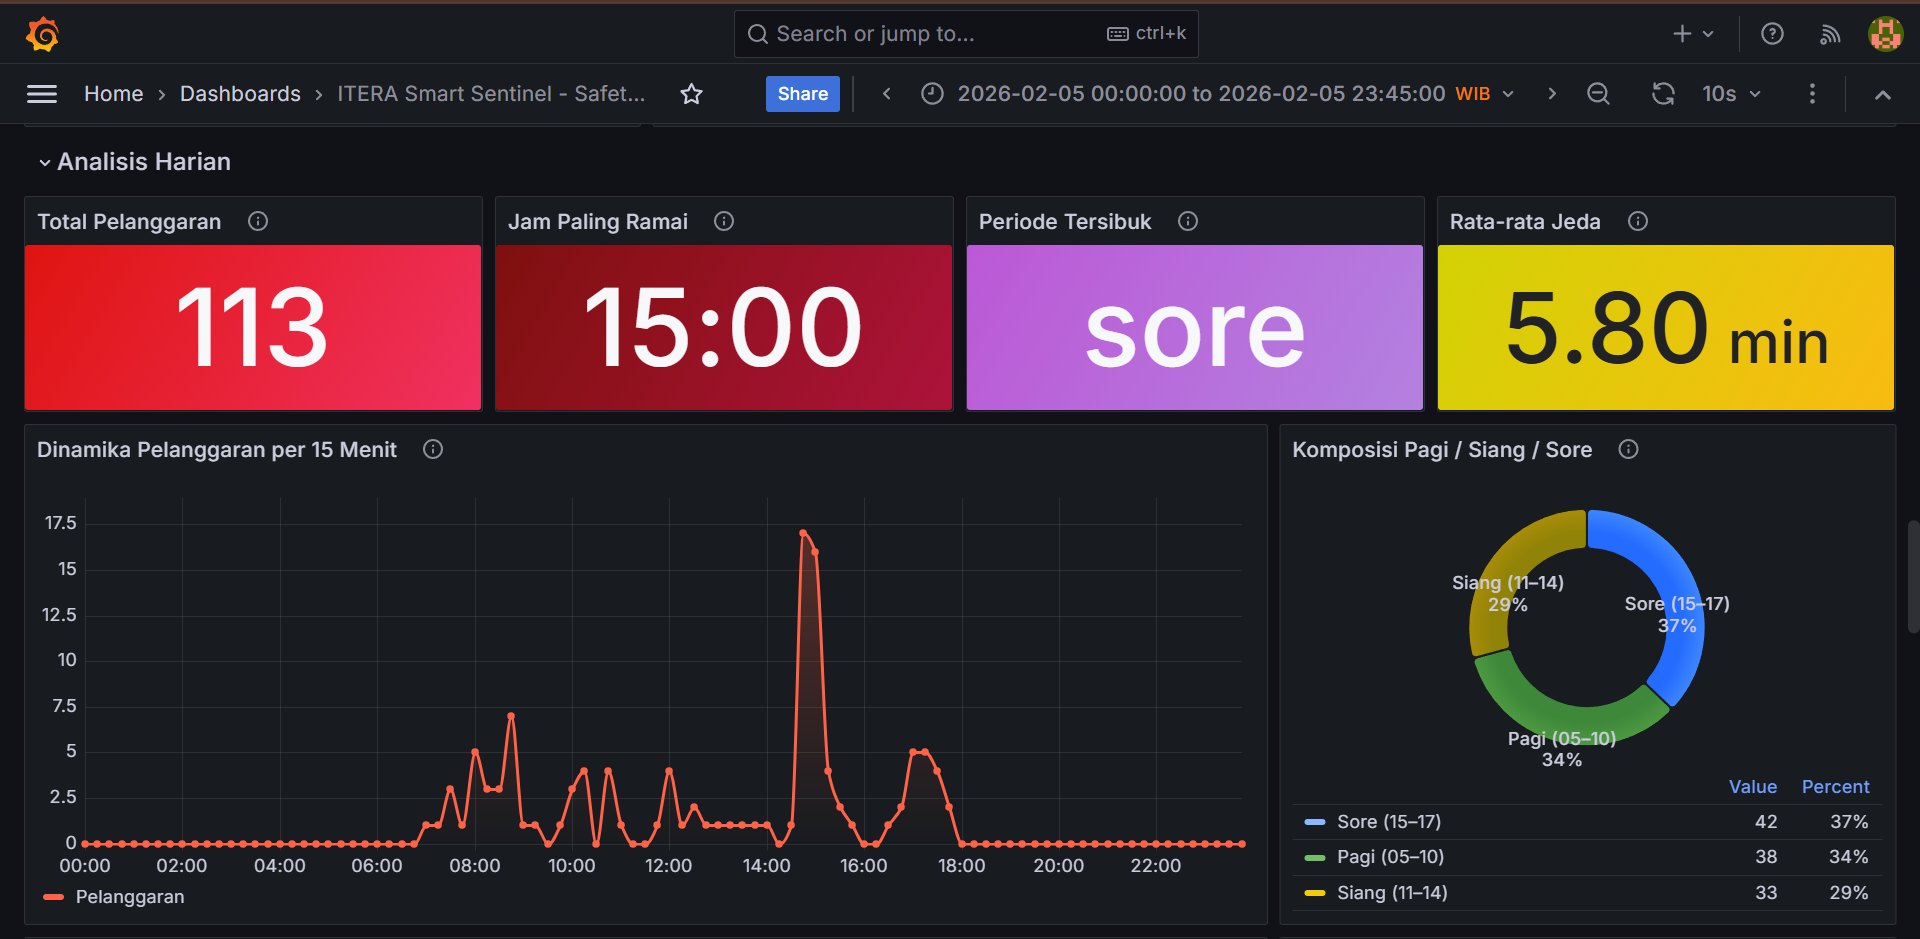
\includegraphics[width=0.95\textwidth]{gambar/grafana_kpi_overview.png}
\caption{Antarmuka utama \textit{dashboard} Grafana untuk data operasional 10 jam: KPI ringkas dan dinamika pelanggaran per 15 menit.}
\label{fig:grafana-kpi-overview}
\end{figure}

% Empat kategori panel disusun supaya operator dapat membaca \textit{dashboard} dari yang paling ringkas ke yang paling rinci. Kategori KPI berada paling atas untuk memberi ringkasan satu pandang, kategori tren waktu mengikuti agar perubahan harian terlihat, kategori performa AI menempati posisi tengah untuk memantau kesehatan model, dan kategori distribusi spasio-temporal di bawah memberi peta panas serta peringkat lokasi rawan. Rincian fungsi tiap kategori ada pada Tabel~\ref{tab:dashboard-panels}.

% Tabel~\ref{tab:dashboard-panels} merangkum peran tiap kategori panel. Kategori \textit{Indikator Kinerja Utama} menempati area paling atas \textit{dashboard} sebagai jendela cepat yang memuat empat metrik agregat dari \texttt{fact\_violations} sekaligus. Kategori \textit{Analisis Dinamika dan Tren Waktu} kemudian membuka detail temporal melalui grafik garis 15 menit, diagram batang akumulasi harian, dan komposisi periode harian. Kategori \textit{Evaluasi Performa Sistem dan AI} memantau dua metrik teknis---probabilitas deteksi dan latensi pemrosesan---yang menjaga kesehatan model di tengah variasi beban. Kategori \textit{Analisis Spasial dan Distribusi Temporal} merangkai matriks peta panas dan peringkat jam tersibuk yang menjawab pertanyaan ``kapan dan di mana pelanggaran paling sering terjadi''. Susunan keempat kategori ini sejalan dengan praktik \textit{drill-down} pada \textit{dashboard} operasional yang mengurutkan informasi dari yang paling agregat ke yang paling rinci.

% Pengujian antarmuka mencatat setiap pembaruan di \texttt{fact\_violations} muncul di panel Grafana dalam beberapa detik. Dengan sinkronisasi yang konsisten, \textit{dashboard} siap dipakai operator gerbang untuk pemantauan harian. Pembacaan pola temporal dan spasial atas data \textit{dashboard} disajikan pada Sub-bab~\ref{subsec:analisis-data-lapangan}.

% Empat kategori panel disusun supaya operator dapat membaca \textit{dashboard} dari yang paling ringkas ke yang paling rinci. Kategori KPI berada paling atas untuk memberi ringkasan satu pandang, kategori tren waktu mengikuti agar perubahan harian terlihat, kategori performa AI menempati posisi tengah untuk memantau kesehatan model, dan kategori distribusi spasio-temporal di bawah memberi peta panas serta peringkat lokasi rawan. Rincian fungsi tiap kategori ada pada Tabel~\ref{tab:dashboard-panels}.


% Pengujian antarmuka mencatat setiap pembaruan di \texttt{fact\_violations} muncul di panel Grafana dalam beberapa detik. Dengan sinkronisasi yang konsisten, \textit{dashboard} siap dipakai operator gerbang untuk pemantauan harian. Pembacaan pola temporal dan spasial atas data \textit{dashboard} disajikan pada Sub-bab~\ref{subsec:analisis-data-lapangan}.

% %  EVIDENCE 2: Tabel Konfigurasi Panel 
% \begin{table}[htbp]
% \centering
% \caption{Kategori panel pada \textit{dashboard} analitik dan fungsinya.}
% \label{tab:dashboard-panels}
% \footnotesize
% \setlength{\tabcolsep}{3pt}
% \renewcommand{\arraystretch}{1.1}
% \begin{tabularx}{\textwidth}{>{\RaggedRight\arraybackslash}p{4cm} >{\RaggedRight\arraybackslash}X}
% \toprule
% \textbf{Kategori Panel} & \textbf{Fungsi} \\
% \midrule
% \textit{Indikator Kinerja Utama (KPI)} & Menyajikan ringkasan indikator secara cepat (\textit{single stat}) di area teratas, meliputi metrik Total Pelanggaran, Jam Paling Ramai, Periode Tersibuk, dan Rata-rata jeda waktu antar-pelanggaran. \\
% \textit{Analisis Dinamika dan Tren Waktu} & Menganalisis fluktuasi \textit{time-series} melalui grafik garis per 15 menit, diagram batang akumulasi pelanggaran sepanjang hari (per jam vs kumulatif), dan komposisi waktu (Pagi/Siang/Sore). \\
% \textit{Evaluasi Performa Sistem dan AI} & Merangkum kestabilan infrastruktur melalui grafik distribusi tingkat keyakinan AI (\textit{confidence level}) dan kecepatan deteksi (\textit{system latency}) saat dihadapkan pada variasi beban data. \\
% \textit{Analisis Spasial dan Distribusi Temporal} & Memvisualisasikan lokasi anomali melalui matriks peta panas (\textit{heatmap}) temporal, sebaran \textit{hotspot} pada peta risiko geospasial, serta ringkasan agregat seperti Peringkat Top 5 Jam Tersibuk. \\
% \bottomrule
% \end{tabularx}
% \renewcommand{\arraystretch}{1.0}
% \end{table}

% % ============================================================
% \subsection{Pola Lapangan dari \textit{Dashboard}}
% \label{subsec:analisis-data-lapangan}
% % ============================================================

% Implementasi \textit{Data Mart} mengekstraksi wawasan operasional dari data lapangan secara berulang. Data yang dipakai adalah hasil inferensi YOLOv8 dari aliran CCTV Kamera Gerbang Utama 1, bukan data sintetis. Pengamatan berlangsung selama 10 jam operasional pada hari kerja (07.00--17.00 WIB). Pembahasan berikut menguraikan keluaran tiap panel \textit{dashboard} untuk menilai peran sistem sebagai pendukung pengambilan keputusan.

% 
\subsubsection{Fluktuasi Pelanggaran per 15 Menit}
\label{subsubsec:analisis-dinamika-15m}

Pada resolusi temporal sempit, sistem mampu mengidentifikasi perubahan volume pelanggaran. Panel grafik garis ``Dinamika Pelanggaran per 15 Menit'' merangkum akumulasi log kejadian dari tabel fakta secara kontinu.

%  EVIDENCE: Potongan gambar dinamika per 15 menit dari grafana_kpi_overview.jpg 
\begin{figure}[htbp]
\centering
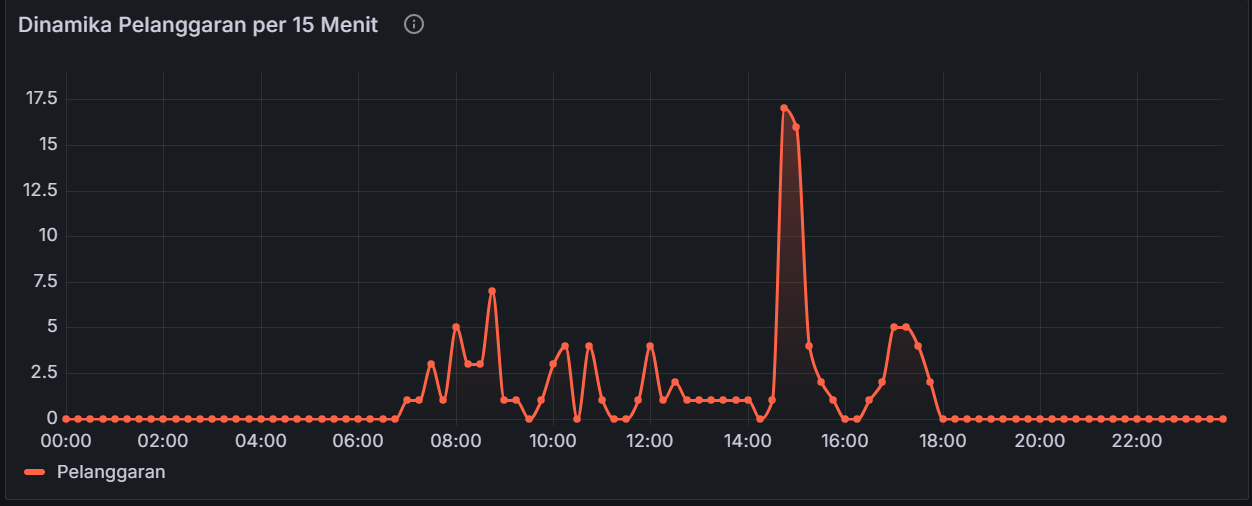
\includegraphics[width=1\textwidth]{gambar/grafana_dinamika_15m.png}
\caption{Fluktuasi pelanggaran per 15 menit. puncak tertinggi 17 kejadian pada kuartal 14.45--15.00 WIB.}
\label{fig:grafana-dinamika-15m}
\end{figure}

Pada Gambar~\ref{fig:grafana-dinamika-15m}, kurva pelanggaran berfluktuasi mengikuti ritme aktivitas kampus. Nilai rendah tercatat pada rentang 09.00--10.00 WIB lalu meningkat tajam saat jam pergantian kelas. Lonjakan tertinggi terjadi pada kuartal 14.45--15.00 WIB dengan 17 kejadian per 15 menit, berbeda jauh dari kuartal-kuartal pagi yang sebagian besar berada di rentang satu hingga tiga kejadian. Kuartal berikutnya, 15.00--15.15 WIB, masih bertahan tinggi dengan 16 kejadian, sehingga periode risiko membentang sekitar 30 menit di sekitar bubaran kelas sore. Observasi lapangan mengaitkan lonjakan tersebut dengan dua kondisi yang berlangsung bersamaan: mobilitas pasca-hujan dan pertemuan arus mahasiswa yang keluar dan masuk kelas.

Resolusi 15 menit menyingkap pulsasi yang tidak teramati pada agregasi per jam, dan justru pulsasi itulah yang seharusnya menjadi sinyal awal bagi operator. Granularitas ini menunjukkan bahwa ketegangan dapat membangun dalam 30--45 menit, jauh sebelum laporan agregat per jam tersedia. Catatan yang perlu disampaikan terbuka: kurva ini berasal dari satu hari pengamatan, sehingga pola tersebut masih perlu dikonfirmasi melalui pengamatan lebih panjang sebelum dipakai sebagai dasar penjadwalan rutin patroli.

% 
\subsubsection{Akumulasi Harian dan Jam Tersibuk}
\label{subsubsec:analisis-akumulasi-jam}

Analisis agregat harian memetakan beban pelanggaran dari waktu ke waktu. Panel grafik Akumulasi Pelanggaran Sepanjang Hari dan matriks Top 5 Jam Tersibuk pada Gambar~\ref{fig:grafana-akumulasi} membandingkan tren kumulatif harian dengan persentase volume tiap jam operasional dalam susunan atas--bawah.

%  EVIDENCE: Potongan gambar bar chart dan top 5 dari grafana_akumulasi_harian.png 
\begin{figure}[htbp]
\centering
\includegraphics[width=0.95\textwidth]{gambar/grafana_akumulasi_harian.png}
\caption{Bagian atas: pertumbuhan kumulatif dan jumlah kejadian per jam. Bagian bawah: peringkat lima jam tersibuk yang terkonsentrasi pada dua periode utama.}
\label{fig:grafana-akumulasi}
\end{figure}

Diagram batang kumulatif (batang biru) menanjak tidak rata sepanjang hari: ada periode dengan lonjakan tajam dan ada periode yang nyaris datar. Dari total 113 kejadian, beban tertinggi tercatat pada pukul 15.00 WIB sebanyak 23 kejadian (20,4\%), diikuti pukul 14.00 WIB sebanyak 19 kejadian (16,8\%), dan pukul 08.00 WIB sebanyak 18 kejadian (15,9\%). Pemusatan beban di tiga jam tersebut membentuk distribusi bimodal: satu puncak pagi dan satu puncak sore, dengan jam kuliah aktif pukul 09.00--11.00 WIB di tengah yang relatif sepi pelanggaran.

Frekuensi kumulatif yang tinggi pada rentang 14.00--15.00 WIB selaras dengan observasi lapangan. Titik kerawanan (\textit{vulnerability point}) jam tersebut bertepatan dengan peningkatan mobilitas mahasiswa setelah hujan lebat reda dan gelombang perpindahan saat transisi kelas sore.

Peringkat jam tersibuk membawa implikasi operasional yang jelas. Unit keamanan kampus dapat memakai distribusi ini untuk menempatkan personel patroli pada jam berisiko tinggi, bukan menyebar rata sepanjang hari. Susunan ini sejalan dengan peran sistem sebagai Sistem Pendukung Keputusan (\textit{Decision Support System}) di tingkat manajerial: data dari kamera berubah menjadi keputusan alokasi sumber daya yang berbasis bukti, bukan dugaan. Pemahaman pola pelanggaran berbasis cuaca dan jadwal kampus juga memungkinkan pengawasan dilakukan lebih awal sebelum jam puncak, sehingga sifatnya menjadi preventif.

% 
\subsubsection{Peta Panas Temporal Kepadatan}
\label{subsubsec:analisis-heatmap}

Pada resolusi waktu yang lebih granular, sistem basis data memproses kueri tabulasi silang (\textit{cross-tabulation}) untuk memetakan anomali kepadatan. Panel ``Peta Panas: Jam $\times$ Kuartal 15 Menit'' pada Gambar~\ref{fig:grafana-heatmap-real} memvisualisasikan distribusi frekuensi kejadian dengan gradasi intensitas warna dan total kumulatif per jam di sisi kanan matriks.

%  EVIDENCE: Potongan gambar heatmap dari grafana_heatmap_real.png 
\begin{figure}[htbp]
\centering
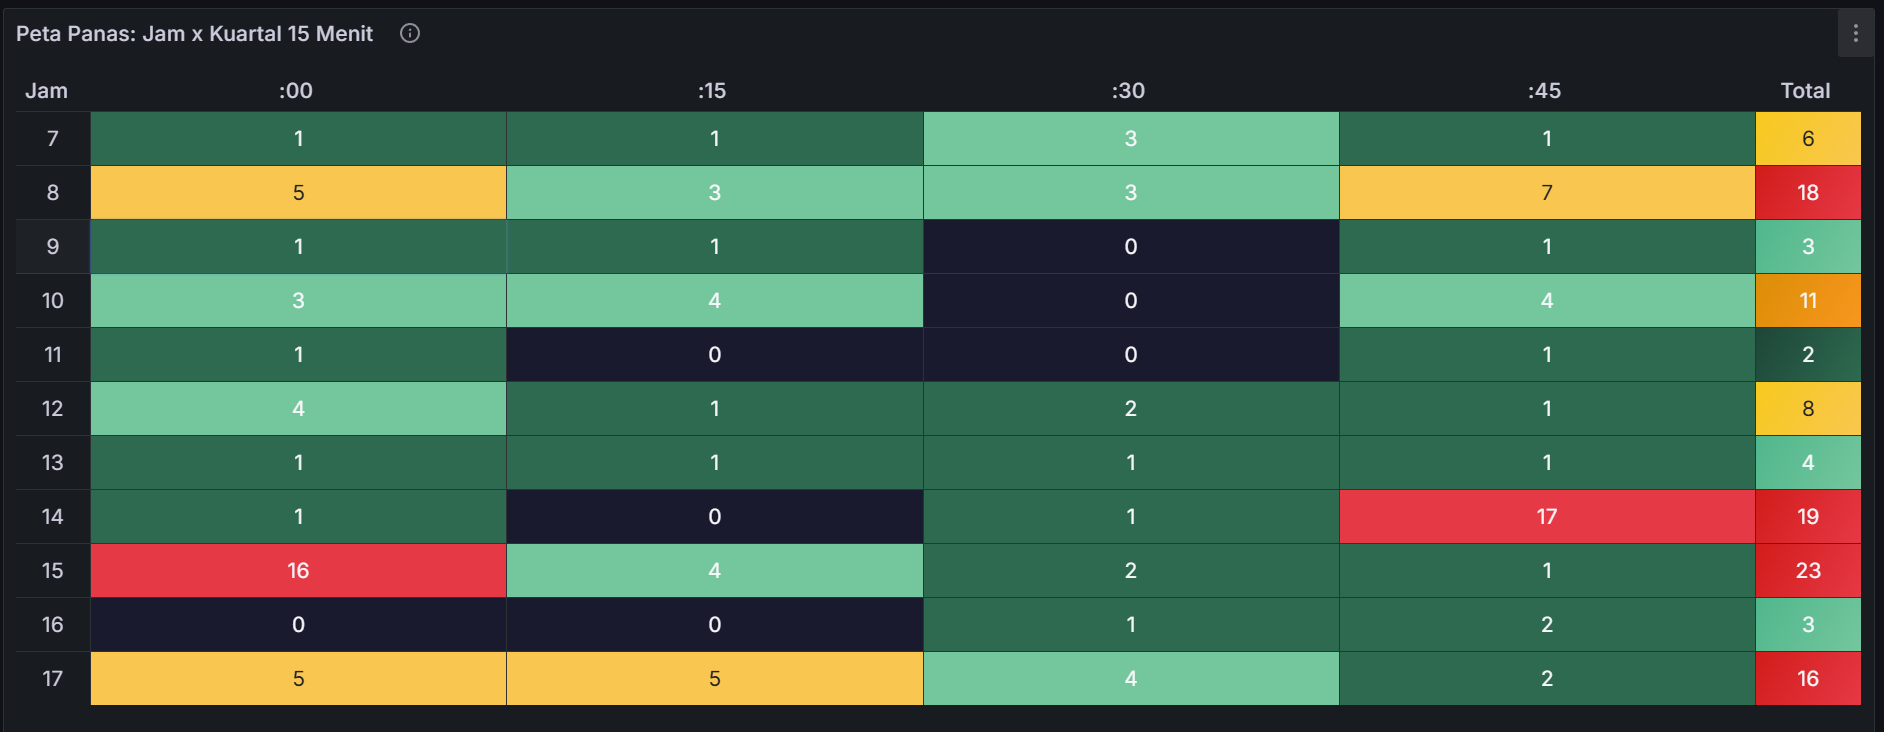
\includegraphics[width=1\textwidth]{gambar/grafana_heatmap_real.png}
\caption{Peta panas kuartal 15 menit. konsentrasi merah pada kolom :45 dan :00 menandai jam rawan pada sore hari.}
\label{fig:grafana-heatmap-real}
\end{figure}

Pada Gambar~\ref{fig:grafana-heatmap-real}, peta panas memperlihatkan fluktuasi waktu yang lebih rinci dibandingkan agregasi per jam. Sumbu vertikal menampung jam 07.00--17.00 WIB, sumbu horizontal memuat empat kuartal (\texttt{:00}, \texttt{:15}, \texttt{:30}, \texttt{:45}), dan gradasi warna dari kuning pucat ke merah pekat menandai intensitas relatif kejadian. Konsentrasi merah pekat sebagai penanda area kerawanan tertinggi (\textit{hotspot}) berkumpul pada jam 14 dan 15, khususnya kuartal \texttt{:45} dan \texttt{:00}. \textit{Dashboard} mencatat 17 kejadian pada kuartal 14.45--15.00 WIB dan 16 kejadian pada kuartal 15.00--15.15 WIB, sehingga periode risiko tinggi membentang sekitar 30 menit di area gerbang kampus.

Pola tersebut selaras dengan peningkatan arus kendaraan sesaat setelah hujan reda yang bertepatan dengan keluarnya mahasiswa dari kelas sore. Sebaliknya, pada jam perkuliahan aktif seperti pukul 11.00 dan 16.00 WIB, intensitas matriks mendekati nol kejadian; ruang putih pada matriks justru dipakai untuk menegaskan kontras dengan zona puncak. Peta panas melengkapi peringkat jam tersibuk pada Sub-bab~\ref{subsubsec:analisis-akumulasi-jam}: peringkat memberi tahu jam mana yang ramai, sementara peta panas memberi tahu kuartal mana di dalam jam tersebut yang paling kritis. Bagi unit keamanan kampus, kombinasi kedua panel cukup untuk memutuskan penempatan personel patroli pada jendela 30 menit yang spesifik, bukan sekadar slot jam yang lebar.

% 
\subsubsection{Stabilitas Inferensi dan Infrastruktur}
\label{subsubsec:analisis-stabilitas-ai}

Bagian terakhir menguji ketahanan (\textit{robustness}) sistem saat aliran data melonjak. Dua hal yang dipantau bersamaan: tingkat keyakinan model YOLOv8 dan latensi infrastruktur saat volume pelanggaran naik. Gambar~\ref{fig:grafana-evaluasi-sistem} memuat dua panel komparasi vertikal dengan batang ungu untuk volume pelanggaran serta kurva untuk \textit{confidence} dan \textit{latency}.


Pada grafik performa AI di bagian atas Gambar~\ref{fig:grafana-evaluasi-sistem}, tingkat keyakinan model bertahan konsisten meski volume pelanggaran melonjak. Saat lonjakan terjadi pada pukul 14.00 dan 15.00 WIB akibat mobilitas pasca-hujan dan pergantian kelas, rata-rata keyakinan (\textit{Avg Confidence}) tetap di kisaran 79,9\% sepanjang hari operasional. Batas bawah keyakinan (\textit{Min Confidence}) tertahan pada 51,2\% tanpa penurunan ekstrem. YOLOv8 dengan demikian tidak mengalami penurunan akurasi saat kepadatan dan oklusi antar-pengendara meningkat akibat cuaca.


%  EVIDENCE: Potongan gambar confidence dan latency dari grafana_evaluasi_sistem.png 
\begin{figure}[htbp]
\centering
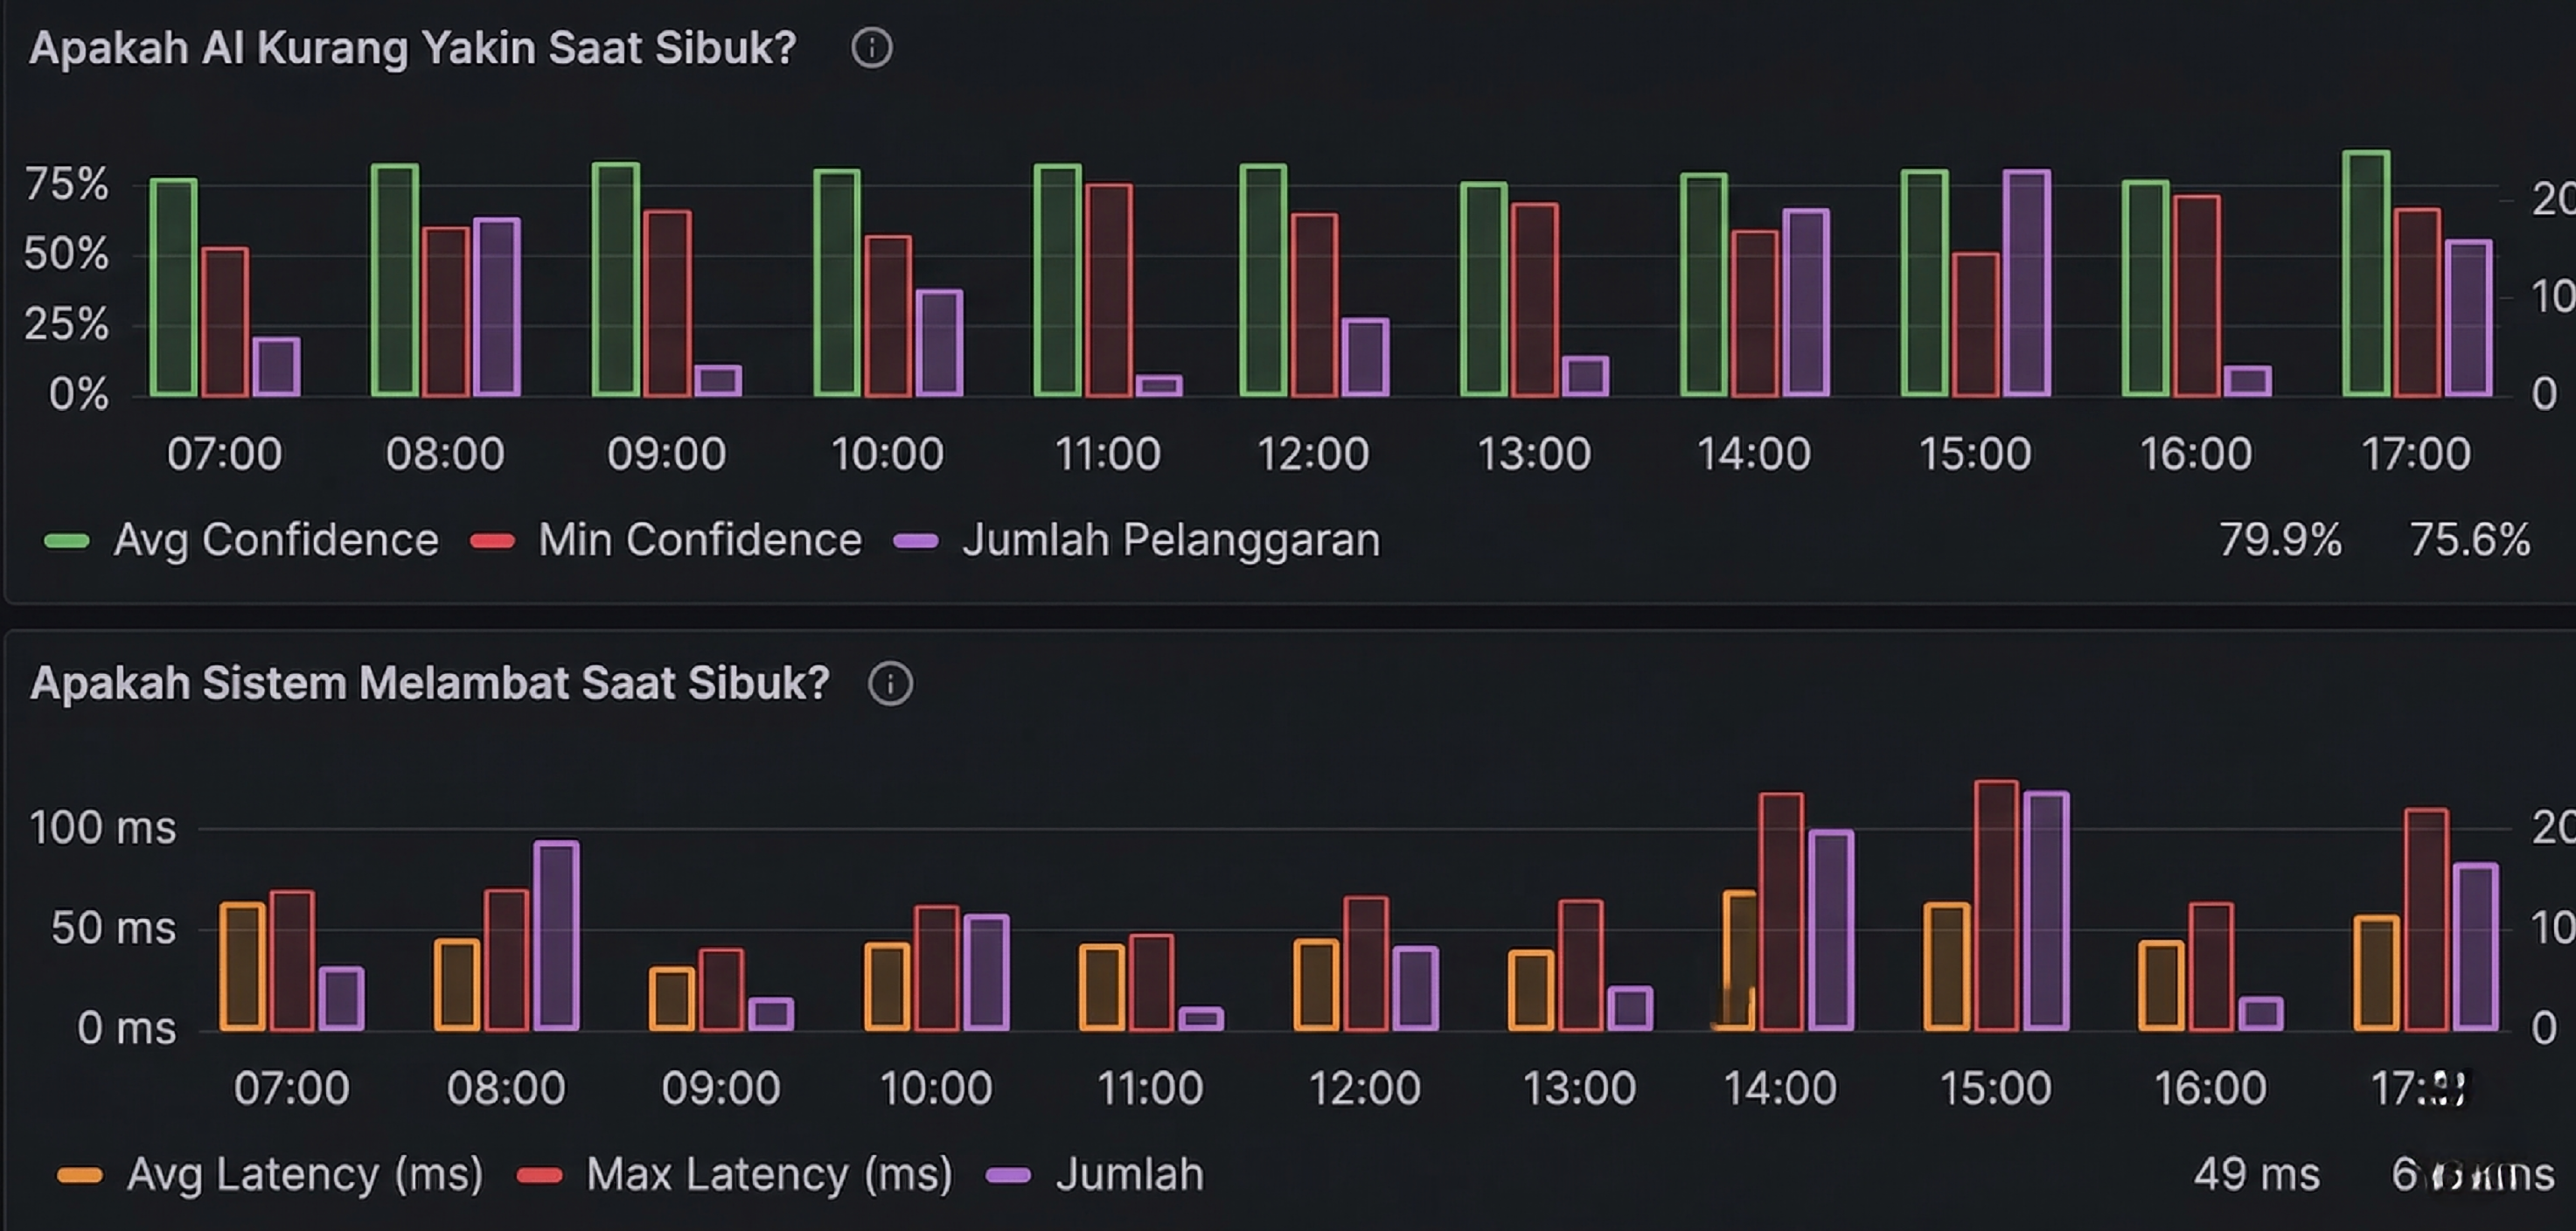
\includegraphics[width=1\textwidth]{gambar/grafana_evaluasi_sistem.png}
\caption{Kinerja arsitektur terhadap lonjakan beban (atas: \textit{confidence} model. bawah: latensi server).}
\label{fig:grafana-evaluasi-sistem}
\end{figure}

Grafik bagian bawah memperlihatkan kinerja infrastruktur komputasi yang tetap stabil meski volume kejadian melonjak. Rata-rata latensi pemrosesan (\textit{Avg Latency}) tercatat 49 milidetik sepanjang sepuluh jam operasional, termasuk pada bubaran kelas sore yang menjadi periode tersibuk. Latensi maksimum (\textit{Max Latency}) sempat naik ke 124 milidetik pada beban puncak (23 kejadian pukul 15.00 WIB), tetapi masih dalam rentang \textit{near real-time} yang dibutuhkan pemantauan CCTV operasional. Selisih antara rata-rata dan maksimum sekitar 2,5 kali lipat, mencerminkan ekor distribusi yang masih wajar dan tidak menunjukkan hambatan kinerja (\textit{bottleneck}) yang menonjol.

Stabilitas tersebut bersumber dari arsitektur yang memisahkan inferensi YOLOv8 di sisi tepi dari distribusi pesan Kafka dan pemrosesan \textit{micro-batch} Spark. Jalur Kafka menampung lonjakan data secara asinkron, sehingga lonjakan trafik di gerbang tidak langsung mempengaruhi waktu respons \textit{pipeline} inferensi. Kombinasi probabilitas yang stabil pada 79,9\% dan latensi yang stabil pada 49 milidetik selama lonjakan beban memperlihatkan sistem dapat dipercaya saat data mengalir deras. Dengan demikian, \textit{data mart} pelanggaran helm dapat dioperasikan secara berkelanjutan tanpa perlu meningkatkan kapasitas perangkat keras setiap kali aktivitas kampus berubah.


% % BAB 5 PENUTUP
% !TEX root = ../main.tex
\chapter{KESIMPULAN DAN SARAN}
\label{chap:kesimpulan}

% ============================================================
\section{Kesimpulan}
\label{sec:kesimpulan}
% ============================================================

Penelitian ini merancang, mengimplementasikan, dan mengevaluasi arsitektur sistem cerdas berbasis komputasi tepi (\textit{edge computing}) dan analitik data besar (\textit{big data analytics}) untuk pelacakan pelanggaran penggunaan helm di Institut Teknologi Sumatera (Itera). Evaluasi kinerja sistem secara menyeluruh menghasilkan tiga kesimpulan utama yang menjawab tujuan penelitian.

\begin{enumerate}[1.]
  \item  Model deteksi objek berbasis YOLOv8 dioptimalkan dengan dataset kustom CCTV kampus dan mencapai \textit{Mean Average Precision} (mAP@50) sebesar 91,4\% pada data validasi serta 90,0\% pada data uji. Selisih marjinal antara \textit{precision} (87,5\%) dan \textit{recall} (86,5\%) memperlihatkan model yang seimbang antara sensitivitas lokalisasi dan presisi pemisahan kelas \texttt{MOTORCYCLE}, \texttt{DRIVER\_HELMET}, dan \texttt{DRIVER\_NO\_HELMET} di tengah variasi distorsi visual dan pencahayaan luar ruang.

  \item Integrasi inferensi YOLOv8 dan pelacakan multiobjek ByteTrack mengubah deteksi piksel mentah menjadi aliran peristiwa (\textit{event stream}) terstruktur. Filter asosiasi spasial (\textit{Intersection over Area}) dan konfirmasi temporal \textit{N-Frame} menggugurkan deteksi positif palsu (\textit{false positives}) sebelum data ditransmisikan. Pada pengujian operasional 10 jam, rangkaian filter tersebut menyaring 11.172 deteksi mentah menjadi 113 \textit{event} pelanggaran yang dipersistenkan ke \textit{data mart}. Arsitektur pemrosesan tepi mencatat \textit{throughput} stabil 18,9 FPS dan latensi inferensi 53 milidetik tanpa dukungan GPU. Distribusi data melalui Apache Kafka (latensi transmisi median 2,65 milidetik) dan Apache Spark Structured Streaming berjalan asinkron tanpa memicu \textit{backpressure} antrian, sehingga sistem tetap stabil pada lonjakan aliran data.

  \item Perancangan \textit{data mart} berbasis skema bintang (\textit{star schema}) pada PostgreSQL menyediakan landasan komputasi untuk \textit{Online Analytical Processing} (OLAP). Pengujian operasional pada data riil selama 10 jam (07.00--17.00 WIB) mengekstraksi wawasan dari 113 kejadian pelanggaran aktual. \textit{Dashboard} Grafana memetakan distribusi kepadatan bimodal, dengan anomali puncak absolut tercatat pada pukul 14.45--15.15 WIB yang berkorelasi dengan faktor cuaca (pasca-hujan deras) dan transisi jadwal kelas. Implementasi infrastruktur ujung-ke-ujung (\textit{end-to-end}) tersebut menempatkan sistem bukan sekadar sebagai alat pendeteksi, melainkan sebagai instrumen Sistem Pendukung Keputusan (\textit{Decision Support System}) yang menggeser pengawasan UPT K3L Itera dari inspeksi reaktif menuju penjagaan preventif berbasis bukti (\textit{data-driven}).
\end{enumerate}

% ============================================================
\section{Saran}
\label{sec:saran}
% ============================================================

Sistem sudah beroperasi sesuai batasan penelitian, namun masih terbuka peluang optimasi agar arsitektur ini siap diterapkan pada skala produksi (\textit{production-grade}). Rekomendasi untuk penelitian lanjutan disusun ke dalam tujuh arah pengembangan berikut.

\begin{enumerate}[1.]
  \item \textbf{Validasi \textit{end-to-end} berbasis pencocokan manual.}
    Evaluasi kinerja sistem saat ini bertumpu pada metrik per komponen (mAP, \textit{throughput}, latensi). Pengembangan ke depan perlu menambahkan validasi \textit{end-to-end} dengan membandingkan \textit{event} keluaran \textit{pipeline} terhadap anotasi manual oleh pengamat manusia pada segmen \textit{peak hour}. Dari pencocokan satu-ke-satu tersebut dapat diturunkan \textit{precision}, \textit{recall}, F1-Score, \textit{counting accuracy}, dan MAPE per jendela 15 menit yang menggambarkan ketepatan sistem sebagai instrumen pencacah pelanggaran, bukan sekadar pendeteksi objek. Praktik pencocokan ini lazim digunakan pada penelitian \textit{video analytics} lapangan dan memperkuat klaim kelayakan operasional.

  \item \textbf{Akselerasi perangkat keras pada simpul tepi (\textit{Edge AI}).}
    Beban inferensi spasial saat ini masih bertumpu pada Unit Pemroses Sentral (CPU). Pengembangan ke arsitektur multikamera (\textit{multi-camera surveillance}) beresolusi tinggi sebaiknya memindahkan inferensi ke akselerator khusus seperti NVIDIA Jetson atau Google Coral \textit{Tensor Processing Unit} (TPU). Akselerator tersebut berpotensi mendorong \textit{throughput} melampaui 30 FPS sekaligus menurunkan latensi operasional secara berarti.

  \item \textbf{Perluasan ekstraksi atribut keselamatan dan identifikasi entitas.}
    Model visi komputer dapat dikembangkan untuk menjangkau pelanggaran sekunder yang juga berkontribusi pada risiko fatalitas, misalnya kelebihan kapasitas penumpang (berbonceng tiga) atau penggunaan ponsel saat berkendara. Integrasi dengan subsistem \textit{Automatic License Plate Recognition} (ALPR) juga relevan agar setiap \textit{event} terikat langsung pada identitas registrasi kendaraan pelanggar dan dapat ditindaklanjuti oleh unit pengamanan kampus.

  \item \textbf{Analitik prediktif dan deteksi dini lonjakan pelanggaran.}
    Catatan operasional 10 jam memperlihatkan pola bimodal pagi--sore yang konsisten dengan jadwal kuliah. Lapisan analitik dapat diperkaya dengan model deret waktu sederhana (mis. SARIMA atau \textit{exponential smoothing}) untuk memproyeksikan lonjakan beban pada jam berikutnya, sehingga UPT K3L menerima peringatan dini sebelum periode rawan dimulai dan dapat menggeser penempatan personel patroli secara proaktif.

  \item \textbf{Penerapan multi-kamera dan fusi sudut pandang.}
    Penelitian ini diuji pada satu kamera gerbang utama. Replikasi pada beberapa titik kritis (gerbang sekunder, persimpangan internal, jalur sepeda motor) bersama mekanisme \textit{re-identification} antar kamera berpeluang memetakan jejak pengendara lintas titik dan mengubah \textit{Track ID} sesi menjadi identitas pelanggar fisik yang persisten---salah satu keterbatasan yang ditandai pada Bab~\ref{chap:hasil}.

  \item \textbf{Penerapan praktik MLOps untuk siklus hidup model.}
    Pelatihan model pada penelitian ini berlangsung satu kali di platform Roboflow Train 3.0, sedangkan operasi produksi memerlukan pembaruan berkelanjutan agar akurasi tidak menurun seiring perubahan musim, sudut kamera, atau ragam kendaraan baru. Penelitian lanjutan dapat membangun jalur MLOps yang menggabungkan registri model (\textit{model registry}), pelacakan versi dataset, dan orkestrasi pelatihan otomatis melalui kakas seperti MLflow, DVC, dan Apache Airflow. Pemantauan pergeseran distribusi (\textit{model drift}) pada keluaran produksi dapat dijalankan dengan kakas seperti Evidently AI atau WhyLabs sehingga pelatihan ulang dipicu otomatis ketika metrik turun di bawah ambang yang ditetapkan. Mekanisme \textit{human-in-the-loop} pada anotasi \textit{event} berkeyakinan rendah menjaga mutu label sekaligus memperkaya dataset secara berkelanjutan, sehingga arsitektur tumbuh dari purwarupa satu kali pelatihan menjadi sistem yang adaptif terhadap perubahan lapangan.

  \item \textbf{Perluasan jalur deteksi ke jenis pelanggaran lalu lintas lain.}
    Sistem saat ini fokus pada pelanggaran helm, namun arsitektur kelas YOLO yang berpasangan dengan filter spasial-temporal sebenarnya siap menampung jenis pelanggaran lain dengan biaya pengembangan yang relatif rendah. Penelitian lanjutan dapat menambahkan jalur deteksi untuk pelanggaran pergerakan seperti melawan arus, motor masuk jalur pejalan kaki, parkir liar di luar petak, dan penerobosan rambu larangan di persimpangan internal kampus. Pelanggaran pergerakan memerlukan analisis lintasan (\textit{trajectory}) lewat \texttt{Track ID} ByteTrack yang dibandingkan terhadap poligon zona dan arah lajur yang ditetapkan operator, bukan asosiasi IoA seperti pada kasus helm. Pengembangan dataset menjadi titik kritis karena setiap kategori membutuhkan anotasi tersendiri; pemanfaatan dataset publik seperti Indian Driving Dataset (IDD) atau dataset CCTV lalu lintas terbuka dapat menjadi \textit{bootstrap} sebelum dataset kampus terkumpul. Dengan struktur yang sama, satu \textit{pipeline} sisi tepi dapat memantau beberapa jenis pelanggaran sekaligus, dan \textit{dashboard} Grafana hanya perlu menambah panel per kategori tanpa mengubah skema bintang \textit{data mart}.
\end{enumerate}

Secara keseluruhan, penelitian ini menyajikan kerangka kerja arsitektur analitik video terintegrasi yang memadukan pembelajaran mendalam (YOLOv8), pelacakan multiobjek (ByteTrack), dan pemrosesan aliran data (Kafka--Spark) sebagai solusi pemantauan keselamatan lalu lintas cerdas di lingkungan perguruan tinggi. Kombinasi modul deteksi, filter spasial-temporal, dan \textit{data mart} bintang menggeser pengawasan helm dari catatan manual menjadi rangkaian \textit{event} terukur yang siap dijadikan basis kebijakan. Ketujuh arah pengembangan di atas membuka jalur kelanjutan agar arsitektur ini tumbuh dari purwarupa satu kamera menjadi infrastruktur kampus yang mandiri dan adaptif.


% DAFTAR PUSTAKA
\phantomsection%<---
\addcontentsline{toc}{chapter}{DAFTAR PUSTAKA}
\sloppy
\printbibliography

% Halaman lampiran di tengah
\newpage
\phantomsection%<---
\addcontentsline{toc}{chapter}{LAMPIRAN}
\input{lainnya/lampiran-di-tengah.tex}

% Lampiran
\begin{appendix}

% !TEX root = ../main.tex
\chapter{LAMPIRAN}

\lampiran{Skema Data Warehouse}
\label{app:star_schema}

\subsubsection{Tabel Fakta (Fact Table)}


\begin{table}[H]
\centering
\caption{Tabel Fakta \textit{f\_violations}}
\label{tab:fact_violations}
\small\setlength{\tabcolsep}{4pt}\begin{tabularx}{\textwidth}{>{\raggedright\arraybackslash}p{0.27\textwidth}>{\raggedright\arraybackslash}p{0.20\textwidth}>{\raggedright\arraybackslash}X}
\toprule
\textbf{Kolom} & \textbf{Tipe Data} & \textbf{Deskripsi} \\
\midrule
\textit{violation\_id} & BIGINT (PK) & Kunci primer unik untuk setiap event pelanggaran. \\
\textit{date\_fk} & INT (FK) & Kunci asing ke \textit{dim\_date} yang menyimpan konteks tanggal kejadian. \\
\textit{camera\_fk} & INT (FK) & Kunci asing ke \textit{dim\_camera}. \\
\textit{violation\_type\_fk} & INT (FK) & Kunci asing ke \textit{dim\_violation\_type}. \\
\textit{track\_id} & VARCHAR(50) & ID unik objek yang dilacak (dari sistem deteksi). \\
\textit{duration\_in\_frame} & INT & Ukuran (measure) durasi objek dalam frame. \\
\bottomrule
\end{tabularx}
\end{table}

\subsubsection{Tabel Dimensi (Dimension Tables)}


\begin{table}[H]
\centering
\caption{Ringkasan Relasi Skema Bintang}
\label{tab:ringkasan-relasi-star-schema}
\small\setlength{\tabcolsep}{4pt}\begin{tabularx}{\textwidth}{>{\raggedright\arraybackslash}p{0.28\textwidth}>{\raggedright\arraybackslash}p{0.24\textwidth}>{\raggedright\arraybackslash}X}
\toprule
\textbf{Tabel} & \textbf{Kunci Utama} & \textbf{Relasi terhadap \textit{fact\_violations}} \\
\midrule
\texttt{dim\_date} & \texttt{date\_pk} & Direlasikan melalui \texttt{date\_fk} untuk menyediakan konteks tanggal kejadian (hari, bulan, tahun, akhir pekan, masa ujian). \\
\texttt{dim\_camera} & \texttt{camera\_pk} & Direlasikan melalui \texttt{camera\_fk} untuk menyediakan konteks sumber kamera dan lokasi pemantauan. \\
\texttt{dim\_violation\_type} & \texttt{type\_pk} & Direlasikan melalui \texttt{violation\_type\_fk} untuk menyediakan konteks jenis pelanggaran yang terdeteksi. \\
\bottomrule
\end{tabularx}
\end{table}

\begin{table}[H]
\centering
\caption{Tabel Dimensi \textit{dim\_date}}
\label{tab:dim_date}
\small\setlength{\tabcolsep}{4pt}\begin{tabularx}{\textwidth}{>{\raggedright\arraybackslash}p{0.27\textwidth}>{\raggedright\arraybackslash}p{0.20\textwidth}>{\raggedright\arraybackslash}X}
\toprule
\textbf{Kolom} & \textbf{Tipe Data} & \textbf{Deskripsi} \\
\midrule
\textit{date\_pk} & INT (PK) & Kunci primer unik untuk dimensi tanggal. \\
\textit{date} & DATE & Tanggal kalender (granularitas baris). \\
\textit{day\_of\_week} & VARCHAR(10) & Nama hari (Senin, Selasa, ...). \\
\textit{month} & SMALLINT & Bulan dalam setahun (1--12). \\
\textit{year} & SMALLINT & Tahun. \\
\textit{is\_weekend} & BOOLEAN & Penanda (True/False) jika akhir pekan. \\
\textit{is\_exam\_period} & BOOLEAN & Penanda (True/False) jika masa ujian. \\
\bottomrule
\end{tabularx}
\end{table}

\begin{table}[H]
\centering
\caption{Tabel Dimensi \textit{dim\_camera}}
\label{tab:dim_camera}
\small\setlength{\tabcolsep}{4pt}\begin{tabularx}{\textwidth}{>{\raggedright\arraybackslash}p{0.27\textwidth}>{\raggedright\arraybackslash}p{0.20\textwidth}>{\raggedright\arraybackslash}X}
\toprule
\textbf{Kolom} & \textbf{Tipe Data} & \textbf{Deskripsi} \\
\midrule
\textit{camera\_pk} & INT (PK) & Kunci primer unik untuk kamera. \\
\textit{camera\_name} & VARCHAR(100) & Nama atau ID kamera (misal: \texttt{CCTV\_GERBANG\_A}). \\
\textit{location\_description} & VARCHAR(255) & Deskripsi lokasi pemasangan CCTV. \\
\textit{gps\_latitude} & DECIMAL(9,6) & Koordinat lintang. \\
\textit{gps\_longitude} & DECIMAL(9,6) & Koordinat bujur. \\
\bottomrule
\end{tabularx}
\end{table}

\begin{table}[H]
\centering
\caption{Tabel Dimensi \textit{dim\_violation\_type}}
\label{tab:dim_violation_type}
\small\setlength{\tabcolsep}{4pt}\begin{tabularx}{\textwidth}{>{\raggedright\arraybackslash}p{0.27\textwidth}>{\raggedright\arraybackslash}p{0.20\textwidth}>{\raggedright\arraybackslash}X}
\toprule
\textbf{Kolom} & \textbf{Tipe Data} & \textbf{Deskripsi} \\
\midrule
\textit{type\_pk} & INT (PK) & Kunci primer unik untuk jenis pelanggaran. \\
\textit{type\_name} & VARCHAR(50) & Nama pelanggaran (misal: \texttt{NO\_HELMET}). \\
\textit{description} & TEXT & Deskripsi detail dari aturan pelanggaran. \\
\bottomrule
\end{tabularx}
\end{table}

\lampiran{Kode Program dan Model melalui QR Code}
\label{app:qr_code_repo}

Lampiran ini menyediakan akses ke kode program dan model penelitian melalui \textit{Quick Response Code} (QR Code) pada Gambar~\ref{fig:qr-code-lampiran} dan tautan klikable \href{https://bit.ly/Lampiran-TA-EGGISATRIA}{lampiran digital}, sehingga pembaca dapat membuka berkas pendukung secara langsung.

\begin{figure}[H]
\centering

\includegraphics[width=0.45\textwidth]{gambar/qr_code_lampiran.png}
\caption{QR Code untuk mengakses lampiran digital yang memuat kode program dan model penelitian.}
\label{fig:qr-code-lampiran}
\end{figure}
\end{appendix}

\end{document}